\documentclass[]{book}
\usepackage{lmodern}
\usepackage{amssymb,amsmath}
\usepackage{ifxetex,ifluatex}
\usepackage{fixltx2e} % provides \textsubscript
\ifnum 0\ifxetex 1\fi\ifluatex 1\fi=0 % if pdftex
  \usepackage[T1]{fontenc}
  \usepackage[utf8]{inputenc}
\else % if luatex or xelatex
  \ifxetex
    \usepackage{mathspec}
  \else
    \usepackage{fontspec}
  \fi
  \defaultfontfeatures{Ligatures=TeX,Scale=MatchLowercase}
\fi
% use upquote if available, for straight quotes in verbatim environments
\IfFileExists{upquote.sty}{\usepackage{upquote}}{}
% use microtype if available
\IfFileExists{microtype.sty}{%
\usepackage{microtype}
\UseMicrotypeSet[protrusion]{basicmath} % disable protrusion for tt fonts
}{}
\usepackage[margin=1in]{geometry}
\usepackage{hyperref}
\hypersetup{unicode=true,
            pdftitle={Exponential random graph models with R},
            pdfauthor={Alberto Caimo and Isabella Gollini},
            pdfborder={0 0 0},
            breaklinks=true}
\urlstyle{same}  % don't use monospace font for urls
\usepackage{natbib}
\bibliographystyle{apalike}
\usepackage{color}
\usepackage{fancyvrb}
\newcommand{\VerbBar}{|}
\newcommand{\VERB}{\Verb[commandchars=\\\{\}]}
\DefineVerbatimEnvironment{Highlighting}{Verbatim}{commandchars=\\\{\}}
% Add ',fontsize=\small' for more characters per line
\usepackage{framed}
\definecolor{shadecolor}{RGB}{248,248,248}
\newenvironment{Shaded}{\begin{snugshade}}{\end{snugshade}}
\newcommand{\KeywordTok}[1]{\textcolor[rgb]{0.13,0.29,0.53}{\textbf{{#1}}}}
\newcommand{\DataTypeTok}[1]{\textcolor[rgb]{0.13,0.29,0.53}{{#1}}}
\newcommand{\DecValTok}[1]{\textcolor[rgb]{0.00,0.00,0.81}{{#1}}}
\newcommand{\BaseNTok}[1]{\textcolor[rgb]{0.00,0.00,0.81}{{#1}}}
\newcommand{\FloatTok}[1]{\textcolor[rgb]{0.00,0.00,0.81}{{#1}}}
\newcommand{\ConstantTok}[1]{\textcolor[rgb]{0.00,0.00,0.00}{{#1}}}
\newcommand{\CharTok}[1]{\textcolor[rgb]{0.31,0.60,0.02}{{#1}}}
\newcommand{\SpecialCharTok}[1]{\textcolor[rgb]{0.00,0.00,0.00}{{#1}}}
\newcommand{\StringTok}[1]{\textcolor[rgb]{0.31,0.60,0.02}{{#1}}}
\newcommand{\VerbatimStringTok}[1]{\textcolor[rgb]{0.31,0.60,0.02}{{#1}}}
\newcommand{\SpecialStringTok}[1]{\textcolor[rgb]{0.31,0.60,0.02}{{#1}}}
\newcommand{\ImportTok}[1]{{#1}}
\newcommand{\CommentTok}[1]{\textcolor[rgb]{0.56,0.35,0.01}{\textit{{#1}}}}
\newcommand{\DocumentationTok}[1]{\textcolor[rgb]{0.56,0.35,0.01}{\textbf{\textit{{#1}}}}}
\newcommand{\AnnotationTok}[1]{\textcolor[rgb]{0.56,0.35,0.01}{\textbf{\textit{{#1}}}}}
\newcommand{\CommentVarTok}[1]{\textcolor[rgb]{0.56,0.35,0.01}{\textbf{\textit{{#1}}}}}
\newcommand{\OtherTok}[1]{\textcolor[rgb]{0.56,0.35,0.01}{{#1}}}
\newcommand{\FunctionTok}[1]{\textcolor[rgb]{0.00,0.00,0.00}{{#1}}}
\newcommand{\VariableTok}[1]{\textcolor[rgb]{0.00,0.00,0.00}{{#1}}}
\newcommand{\ControlFlowTok}[1]{\textcolor[rgb]{0.13,0.29,0.53}{\textbf{{#1}}}}
\newcommand{\OperatorTok}[1]{\textcolor[rgb]{0.81,0.36,0.00}{\textbf{{#1}}}}
\newcommand{\BuiltInTok}[1]{{#1}}
\newcommand{\ExtensionTok}[1]{{#1}}
\newcommand{\PreprocessorTok}[1]{\textcolor[rgb]{0.56,0.35,0.01}{\textit{{#1}}}}
\newcommand{\AttributeTok}[1]{\textcolor[rgb]{0.77,0.63,0.00}{{#1}}}
\newcommand{\RegionMarkerTok}[1]{{#1}}
\newcommand{\InformationTok}[1]{\textcolor[rgb]{0.56,0.35,0.01}{\textbf{\textit{{#1}}}}}
\newcommand{\WarningTok}[1]{\textcolor[rgb]{0.56,0.35,0.01}{\textbf{\textit{{#1}}}}}
\newcommand{\AlertTok}[1]{\textcolor[rgb]{0.94,0.16,0.16}{{#1}}}
\newcommand{\ErrorTok}[1]{\textcolor[rgb]{0.64,0.00,0.00}{\textbf{{#1}}}}
\newcommand{\NormalTok}[1]{{#1}}
\usepackage{longtable,booktabs}
\usepackage{graphicx,grffile}
\makeatletter
\def\maxwidth{\ifdim\Gin@nat@width>\linewidth\linewidth\else\Gin@nat@width\fi}
\def\maxheight{\ifdim\Gin@nat@height>\textheight\textheight\else\Gin@nat@height\fi}
\makeatother
% Scale images if necessary, so that they will not overflow the page
% margins by default, and it is still possible to overwrite the defaults
% using explicit options in \includegraphics[width, height, ...]{}
\setkeys{Gin}{width=\maxwidth,height=\maxheight,keepaspectratio}
\IfFileExists{parskip.sty}{%
\usepackage{parskip}
}{% else
\setlength{\parindent}{0pt}
\setlength{\parskip}{6pt plus 2pt minus 1pt}
}
\setlength{\emergencystretch}{3em}  % prevent overfull lines
\providecommand{\tightlist}{%
  \setlength{\itemsep}{0pt}\setlength{\parskip}{0pt}}
\setcounter{secnumdepth}{5}
% Redefines (sub)paragraphs to behave more like sections
\ifx\paragraph\undefined\else
\let\oldparagraph\paragraph
\renewcommand{\paragraph}[1]{\oldparagraph{#1}\mbox{}}
\fi
\ifx\subparagraph\undefined\else
\let\oldsubparagraph\subparagraph
\renewcommand{\subparagraph}[1]{\oldsubparagraph{#1}\mbox{}}
\fi

%%% Use protect on footnotes to avoid problems with footnotes in titles
\let\rmarkdownfootnote\footnote%
\def\footnote{\protect\rmarkdownfootnote}

%%% Change title format to be more compact
\usepackage{titling}

% Create subtitle command for use in maketitle
\newcommand{\subtitle}[1]{
  \posttitle{
    \begin{center}\large#1\end{center}
    }
}

\setlength{\droptitle}{-2em}
  \title{Exponential random graph models with R}
  \pretitle{\vspace{\droptitle}\centering\huge}
  \posttitle{\par}
  \author{Alberto Caimo and Isabella Gollini}
  \preauthor{\centering\large\emph}
  \postauthor{\par}
  \predate{\centering\large\emph}
  \postdate{\par}
  \date{2017-04-10}

\usepackage{booktabs}
\usepackage{amsthm}
\makeatletter
\def\thm@space@setup{%
  \thm@preskip=8pt plus 2pt minus 4pt
  \thm@postskip=\thm@preskip
}
\makeatother

\begin{document}
\maketitle

{
\setcounter{tocdepth}{1}
\tableofcontents
}
\chapter*{Preface}\label{preface}
\addcontentsline{toc}{chapter}{Preface}

Interest in statistical network analysis has grown massively in recent
decades and its perspective and methods are now widely used in many
scientific areas which involve the study of various types of networks
for representing structure in many complex relational systems such as
social relationships, information flows, protein interactions.

This manual is written for students in statistical network analysis
courses as well as for people already engaged in these fields. Our aim
is to offer the reader a balanced presentation of the fundamental
statistical concepts and methods and practical advice on their effective
implementation using R.

\section*{About the authors}\label{about-the-authors}
\addcontentsline{toc}{section}{About the authors}

\subsection*{Alberto Caimo}\label{alberto-caimo}
\addcontentsline{toc}{subsection}{Alberto Caimo}

Alberto Caimo is a lecturer in Statistics in the School of Mathematical
Sciences at the Dublin Institute of Technology, Ireland. His current
research activity concerns the development and implementation of
statistical modelling and computational approaches for complex
relational data in a wide variety of applications involving
interdisciplinary collaborations. Alberto is the author of the R package
\href{https://CRAN.R-project.org/package=Bergm}{\texttt{Bergm}} for the
analysis of Bayesian exponential random graph models.

More info:
\href{https://sites.google.com/site/albertocaimo/}{https://sites.google.com/site/albertocaimo}

\subsection*{Isabella Gollini}\label{isabella-gollini}
\addcontentsline{toc}{subsection}{Isabella Gollini}

Isabella Gollini is a lecturer in Statistics in the Department of
Economics, Mathematics and Statistics at the Birkbeck, University of
London, UK. Her research activity focuses on cutting-edge statistical
topics in the area of statistical modelling and computational
statistics. Isabella is the leader of the teaching team of
\href{http://forwards.github.io/}{Forwards: the R Foundation taskforce
on women and under-represented groups}, and she is the author of several
R packages, including
\href{https://CRAN.R-project.org/package=lvm4net}{\texttt{lvm4net}} for
the analysis of latent variable models for network data using fast
inferential procedures.

More info:
\href{https://sites.google.com/site/isabellagollini/}{https://sites.google.com/site/isabellagollini}

\chapter{Introduction}\label{intro}

Social network theory is based on the study of social relations between
actors so as to understand the formation of social structures by the
analysis of basic local relations. Statistical models have started to
play an increasingly important role because they give the possibility to
explain the complexity of social behaviour and to investigate issues on
how the global features of an observed network may be related to local
network structures. The observed network is assumed to be generated by
local social processes which depend on the self-organizing dyadic
relations between actors.

The crucial challenge for statistical models in social network theory is
to capture and describe the dependency giving rise to network global
topology allowing inference about whether certain local structures are
more common than expected.

Exponential random graph models (ERGMs) \citep{hol:lei81} are an
important family of models conceived to capture the complex dependence
structure of an observed network allowing a reasonable interpretation of
the underlying process which is supposed to have produced these
structural properties. The dependence hypothesis at the basis of these
models is that the connections between actors (edges) self-organize into
small structures called configurations or network statistics. These are
classical graph-theoretic structures such as degrees, cycles, etc. which
can be directly incorporated in ERGMs as sufficient statistics with
corresponding parameters measuring their importance in the observed
network.

The computational intractability of ERGMs is the main barrier to
estimation. Fortunately, recent theoretical developments and advanced
computational procedures have given the possibility to make important
progress to overcome statistical inference problems.

\chapter{R basics}\label{Rbasics}

R is an open source programming language and software environment for
statistical computing and graphics that is supported by the R Foundation
for Statistical Computing \citep{R}.

\section{Fundamentals}\label{fundamentals}

\begin{itemize}
\tightlist
\item
  R uses a command-like environment
\item
  R is highly extendable
\item
  You can write your own custom functions
\item
  There are more than 10,000 free packages
\item
  Generally good at reading in/writing out other file formats
\item
  Everything in R is an \textbf{object}
\end{itemize}

\section{R and RStudio}\label{r-and-rstudio}

To install R on your computer, go to the home of the R website at
\url{https://www.r-project.org/}.

We recommend to use the RStudio interface. To install RStudio, go to:
\url{http://www.rstudio.org/}.

\section{Package repositories}\label{package-repositories}

In R, the fundamental unit of shareable code is the package. A package
bundles together code, data, documentation, and tests, and is easy to
share with others. Most packages are stored, in an organized way, in
online repositories from which they can be easily retrieved and
installed on your computer.

There are two main R repositories:

\begin{itemize}
\tightlist
\item
  The Comprehensive R Archive Network (CRAN):
  \url{https://cran.r-project.org/}.
\item
  Bioconductor (open source software for bioinformatics):
  \url{https://www.bioconductor.org/}.
\end{itemize}

\section{R packages for statistical network
analysis}\label{r-packages-for-statistical-network-analysis}

\subsection{\texorpdfstring{\texttt{statnet}}{statnet}}\label{statnet}

\texttt{statnet} \citep{statnet} is a suite of software packages
providing a comprehensive framework based on exponential random graph
models, including tools for model estimation, model evaluation,
model-based network simulation, and network visualization.

More info: \url{https://CRAN.R-project.org/package=statnet}.

\subsection{\texorpdfstring{\texttt{Bergm}}{Bergm}}\label{bergm}

The \texttt{Bergm} package \citep{cai:fri14} provides a comprehensive
framework for Bayesian estimation of exponential random graph models. It
can also supply graphical Bayesian goodness-of-fit procedures that
address the issue of model adequacy.

More info: \url{https://CRAN.R-project.org/package=Bergm}.

\chapter{The random graph model}\label{RGM}

\section{Networks as random graphs}\label{networks-as-random-graphs}

We describe as the observed network the network data the researcher has
collected and is interested in modeling. The observed network is
regarded as one realization from a set of possible networks with similar
important features, that is, as the outcome of some (unknown) stochastic
process. In other words, the observed network is seen as one particular
pattern of edges out of a large set of possible patterns.

Network data are generally represented by graphs of nodes (actors) and
edges (relations). Social network analysis focuses on the relations
among actors, and not individual actors and their attributes. In fact,
for a given model, the node set is regarded as fixed. The range of
possible networks, and their probability of occurrence under the model,
is represented by a probability distribution on the set of all possible
graphs with this number of nodes.

Once we have defined a probability distribution on the set of all graphs
with a fixed number of nodes, we can also draw graphs at random from the
distribution according to their assigned probabilities, and we can
compare the sampled graphs to the observed one on any other
characteristic of interest. If the model is a good one for the data,
then the sampled graphs will resemble the observed one in many different
respects.

\subsection{Notation}\label{notation}

\begin{itemize}
\tightlist
\item
  \(N\) number of nodes (\textbf{fixed}).
\item
  \(D\) number of dyads in a \(N\)-node network (\textbf{fixed}).
\item
  \(Y\) \textbf{random} \(N \times N\) adjacency matrix
  \(\in \mathcal{Y}\) where:

  \begin{itemize}
  \tightlist
  \item
    \(Y_{ij} = 0\), if \(i\) and \(j\) are not connected;
  \item
    \(Y_{ij} = 1\), if \(i\) and \(j\) are connected;
  \item
    \(Y_{ii} = 0\), (self-loops are not allowed).
  \end{itemize}
\item
  \(y\) realisation of \(Y\) (observed adjacency matrix).
\end{itemize}

\(Y\) may be directed so \(Y_{ij}\) and \(Y_{ji}\) are two different
random variables observed between the same pair of nodes.

Let's create a random network on 13 nodes using the \texttt{network}
function and have a look at the corresponding adjacency matrix:

\begin{Shaded}
\begin{Highlighting}[]
\KeywordTok{library}\NormalTok{(statnet)}
\KeywordTok{set.seed}\NormalTok{(}\DecValTok{11}\NormalTok{)}
\NormalTok{N <-}\StringTok{ }\DecValTok{13}
\NormalTok{y <-}\StringTok{ }\KeywordTok{network}\NormalTok{(N, }\DataTypeTok{directed =} \OtherTok{FALSE}\NormalTok{)}
\NormalTok{y[,]}
\end{Highlighting}
\end{Shaded}

\begin{verbatim}
##    1 2 3 4 5 6 7 8 9 10 11 12 13
## 1  0 0 1 1 1 0 0 0 1  0  0  0  1
## 2  0 0 0 1 0 0 0 0 0  1  0  0  0
## 3  1 0 0 0 0 0 0 0 0  0  1  0  0
## 4  1 1 0 0 1 0 1 1 0  1  0  1  0
## 5  1 0 0 1 0 0 0 0 0  0  0  0  0
## 6  0 0 0 0 0 0 0 0 0  0  0  1  0
## 7  0 0 0 1 0 0 0 1 0  0  0  0  0
## 8  0 0 0 1 0 0 1 0 0  0  0  0  0
## 9  1 0 0 0 0 0 0 0 0  0  0  0  0
## 10 0 1 0 1 0 0 0 0 0  0  0  0  0
## 11 0 0 1 0 0 0 0 0 0  0  0  0  0
## 12 0 0 0 1 0 1 0 0 0  0  0  0  0
## 13 1 0 0 0 0 0 0 0 0  0  0  0  0
\end{verbatim}

\subsection{Visualisation}\label{visualisation}

Let's have a look at the network graph:

\begin{Shaded}
\begin{Highlighting}[]
\KeywordTok{set.seed}\NormalTok{(}\DecValTok{11}\NormalTok{)}
\KeywordTok{plot}\NormalTok{(y, }\DataTypeTok{vertex.cex =} \DecValTok{2}\NormalTok{, }\DataTypeTok{vertex.col =} \StringTok{"skyblue"}\NormalTok{, }\DataTypeTok{label =} \KeywordTok{seq}\NormalTok{(}\DecValTok{1}\NormalTok{, N))}
\end{Highlighting}
\end{Shaded}

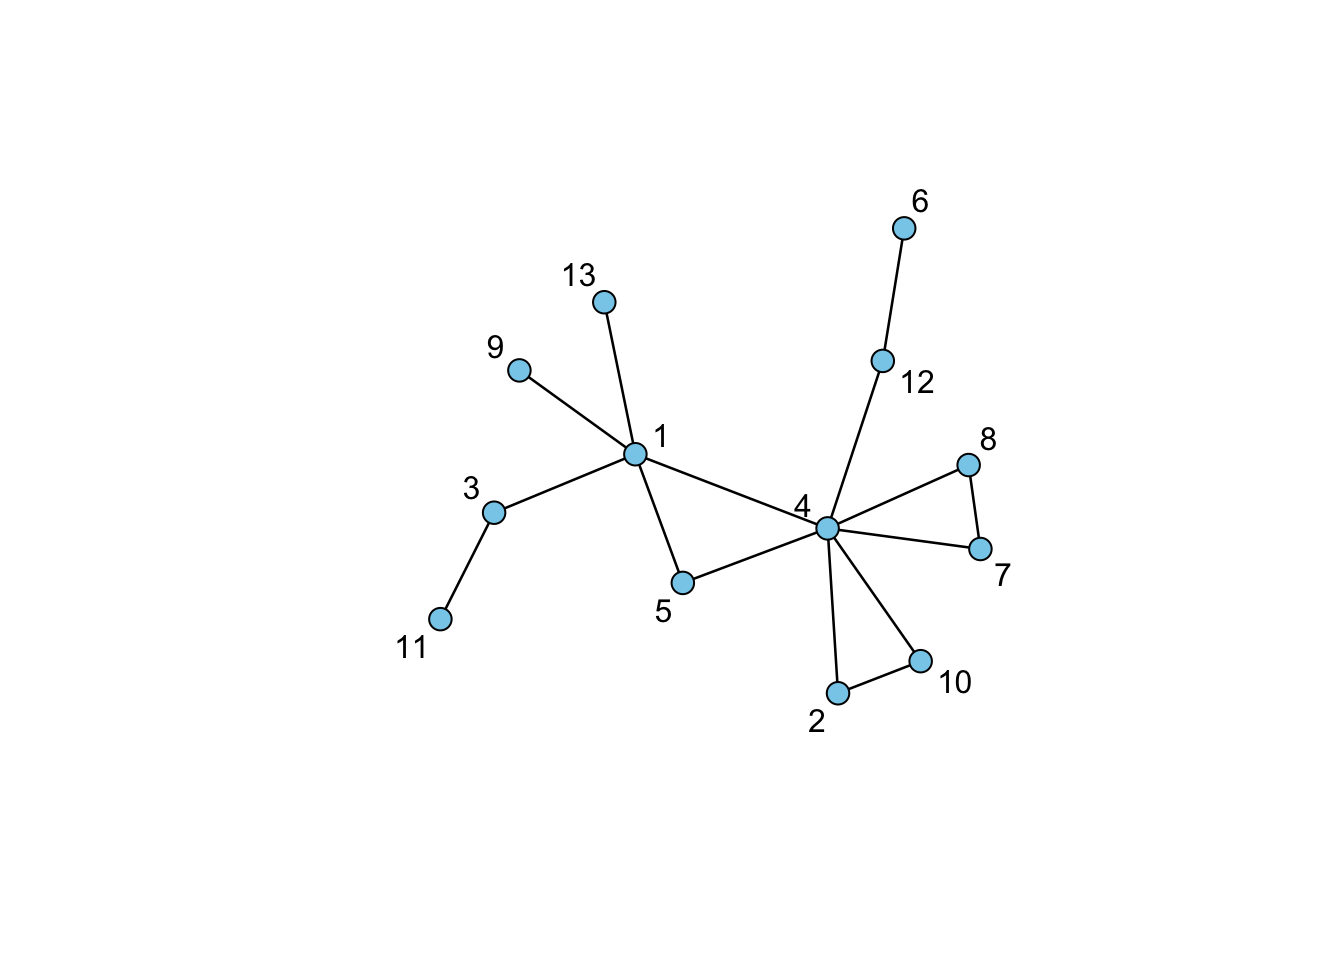
\includegraphics{SNA_BOOK_files/figure-latex/unnamed-chunk-2-1.pdf}

\subsection{Number of dyads}\label{number-of-dyads}

In an undirected graph, we have: \[
D = \frac{N^2 - N}{2}
\]

\begin{Shaded}
\begin{Highlighting}[]
\NormalTok{D <-}\StringTok{ }\NormalTok{(N^}\DecValTok{2} \NormalTok{-}\StringTok{ }\NormalTok{N) /}\StringTok{ }\DecValTok{2}
\NormalTok{D}
\end{Highlighting}
\end{Shaded}

\begin{verbatim}
## [1] 78
\end{verbatim}

\subsection{Number of edges}\label{number-of-edges}

The number of edges is the sum of the 1's in the observed adjacency
matrix \(y\): \[
E = s_1(y) = \sum_{i < j} y_{ij}.
\]

For an undirected adjacency matrix (like \(y\)), we have:

\begin{Shaded}
\begin{Highlighting}[]
\NormalTok{s1 <-}\StringTok{ }\KeywordTok{sum}\NormalTok{(y[,]) /}\StringTok{ }\DecValTok{2}\NormalTok{; s1}
\end{Highlighting}
\end{Shaded}

\begin{verbatim}
## [1] 15
\end{verbatim}

or using the \texttt{summary} function included in the \texttt{ergm}
package:

\begin{Shaded}
\begin{Highlighting}[]
\NormalTok{s1 <-}\StringTok{ }\KeywordTok{summary}\NormalTok{(y ~}\StringTok{ }\NormalTok{edges); s1}
\end{Highlighting}
\end{Shaded}

\begin{verbatim}
## edges 
##    15
\end{verbatim}

The \texttt{summary} function can be used to get general information
about the network:

\begin{Shaded}
\begin{Highlighting}[]
\KeywordTok{summary}\NormalTok{(y)}
\end{Highlighting}
\end{Shaded}

\begin{verbatim}
## Network attributes:
##   vertices = 13
##   directed = FALSE
##   hyper = FALSE
##   loops = FALSE
##   multiple = FALSE
##   bipartite = FALSE
##  total edges = 15 
##    missing edges = 0 
##    non-missing edges = 15 
##  density = 0.1923077 
## 
## Vertex attributes:
##   vertex.names:
##    character valued attribute
##    13 valid vertex names
## 
## No edge attributes
## 
## Network adjacency matrix:
##    1 2 3 4 5 6 7 8 9 10 11 12 13
## 1  0 0 1 1 1 0 0 0 1  0  0  0  1
## 2  0 0 0 1 0 0 0 0 0  1  0  0  0
## 3  1 0 0 0 0 0 0 0 0  0  1  0  0
## 4  1 1 0 0 1 0 1 1 0  1  0  1  0
## 5  1 0 0 1 0 0 0 0 0  0  0  0  0
## 6  0 0 0 0 0 0 0 0 0  0  0  1  0
## 7  0 0 0 1 0 0 0 1 0  0  0  0  0
## 8  0 0 0 1 0 0 1 0 0  0  0  0  0
## 9  1 0 0 0 0 0 0 0 0  0  0  0  0
## 10 0 1 0 1 0 0 0 0 0  0  0  0  0
## 11 0 0 1 0 0 0 0 0 0  0  0  0  0
## 12 0 0 0 1 0 1 0 0 0  0  0  0  0
## 13 1 0 0 0 0 0 0 0 0  0  0  0  0
\end{verbatim}

\section{Random graph model}\label{random-graph-model}

\textbf{Definition} - The likelihood of a random graph model represents
the probability distribution of a network graph \(y\) given a parameter
\(\eta\): \[
p(y\ |\ \eta) = \prod_{i < j} \eta^{y_{ij}}(1-\eta)^{1-y_{ij}} = \eta^{s_1(y)}(1 - \eta)^{D - s_1(y)}
\] where \(0 \le \eta \le 1\).

\subsection{Estimation}\label{estimation}

To estimate \(\eta\) we can just calculate the \textbf{density} of the
network, i.e., the proportion of edges: \[
\hat{\eta} = \frac{s_1(y)}{D}: 
\]

\begin{Shaded}
\begin{Highlighting}[]
\NormalTok{eta <-}\StringTok{ }\NormalTok{s1 /}\StringTok{ }\NormalTok{D; eta}
\end{Highlighting}
\end{Shaded}

\begin{verbatim}
##     edges 
## 0.1923077
\end{verbatim}

this is equivalent to:

\begin{Shaded}
\begin{Highlighting}[]
\NormalTok{eta <-}\StringTok{ }\KeywordTok{summary}\NormalTok{(y ~}\StringTok{ }\NormalTok{density); eta}
\end{Highlighting}
\end{Shaded}

\begin{verbatim}
##   density 
## 0.1923077
\end{verbatim}

\subsection{Natural parametrisation}\label{natural-parametrisation}

Now consider \(\theta = \mathrm{logit}(\eta)\): \[
\eta = \frac{\exp \{ \theta \} }{1 + \exp \{ \theta \}},
\] then the random graph model can be written as an exponential family
distribution: \[
p(y\ |\ \theta) = \prod_{i < j}
\frac{\exp \left\lbrace \theta \right\rbrace^{y_{ij}}}
     {1 + \exp \left\lbrace \theta \right\rbrace}
=
\frac{\exp\left\lbrace \theta^t\ s_1(y) \right\rbrace}
     {c(\theta)}
\] where \(-\infty < \theta < +\infty\) and \[
c(\theta) 
=
\sum_{y' \in \mathcal{Y}} \exp\left\lbrace \theta^t\ s_1(y') \right\rbrace
\] is a normalising constant.

Let's get an estimate of \(\theta\) using the \texttt{ergm} function:

\begin{Shaded}
\begin{Highlighting}[]
\NormalTok{theta <-}\StringTok{ }\KeywordTok{ergm}\NormalTok{(y ~}\StringTok{ }\NormalTok{edges); theta$coef}
\end{Highlighting}
\end{Shaded}

\begin{verbatim}
## Evaluating log-likelihood at the estimate.
\end{verbatim}

\begin{verbatim}
##     edges 
## -1.435085
\end{verbatim}

Let's check whether
\(\dfrac{\exp \{ \hat{\theta} \} }{1 + \exp \{ \hat{\theta} \}} = \hat{\eta}:\)

\begin{Shaded}
\begin{Highlighting}[]
\KeywordTok{round}\NormalTok{(}\KeywordTok{exp}\NormalTok{(theta$coef) /}\StringTok{ }\NormalTok{(}\DecValTok{1} \NormalTok{+}\StringTok{ }\KeywordTok{exp}\NormalTok{(theta$coef)), }\DecValTok{4}\NormalTok{) ==}\StringTok{ }\KeywordTok{round}\NormalTok{(eta, }\DecValTok{4}\NormalTok{)}
\end{Highlighting}
\end{Shaded}

\begin{verbatim}
## edges 
##  TRUE
\end{verbatim}

\subsection{Parameter interpretation}\label{parameter-interpretation}

The parameter estimate \(\theta\) provide insights about the
contribution of the edge statistic \(s_1(y)\) to edge formation.

When \(\theta = 0\), probability of observing an edge between two nodes
\(i\) and \(j\) is:

\begin{equation*}
\Pr(Y_{ij} = 1\ |\ \theta = 0) = \frac{\exp \{ 0 \} }{ 1 + \exp \{ 0 \} } = \eta = 0.5.
\end{equation*}

where \(Y_{ij}\) is an node pair in \(Y\) and \(Y_{-ij}\) is the rest of
the network.

A negative (positive) value of \(\theta\) means that the probability of
observing a network with a higher number of edges is lower (higher) than
the probability of observing a network whose probability of observing an
edge between two nodes is \(0.5\):
\[\Pr(Y_{ij} = 1\ |\ \theta < 0) = \eta < 0.5,\]
\[\Pr(Y_{ij} = 1\ |\ \theta > 0) = \eta > 0.5.\]

Let's take a look at the summary of model fit using the \texttt{summary}
function:

\begin{Shaded}
\begin{Highlighting}[]
\KeywordTok{summary}\NormalTok{(theta)}
\end{Highlighting}
\end{Shaded}

\begin{verbatim}
## 
## ==========================
## Summary of model fit
## ==========================
## 
## Formula:   y ~ edges
## 
## Iterations:  5 out of 20 
## 
## Monte Carlo MLE Results:
##       Estimate Std. Error MCMC % p-value    
## edges  -1.4351     0.2873      0  <1e-04 ***
## ---
## Signif. codes:  0 '***' 0.001 '**' 0.01 '*' 0.05 '.' 0.1 ' ' 1
## 
##      Null Deviance: 108.13  on 78  degrees of freedom
##  Residual Deviance:  76.37  on 77  degrees of freedom
##  
## AIC: 78.37    BIC: 80.73    (Smaller is better.)
\end{verbatim}

In this example, \(\theta \approx -1.4351\) corresponding to
\(\eta \approx 0.1923\). So we can conclude that the network is
\emph{sparse} as the probability to observe an edge connecting any pair
of nodes is about 20\%.

\section{Network simulation}\label{network-simulation}

The estimate \(\hat{\eta}\) is the probability of observing an edge
between any pair of nodes in our \(N\)-node network.

To simulate from the estimated random graph model we can simply simulate
\(N \times N - N\) Bernoulli trials and arrange them into a
\(N \times N\) adjacency matrix:

\begin{Shaded}
\begin{Highlighting}[]
\KeywordTok{set.seed}\NormalTok{(}\DecValTok{11}\NormalTok{)}
\NormalTok{adj.sim <-}\StringTok{ }\KeywordTok{matrix}\NormalTok{(}\KeywordTok{rbinom}\NormalTok{(N *}\StringTok{ }\NormalTok{N, }\DataTypeTok{size =} \DecValTok{1}\NormalTok{, }\DataTypeTok{prob =} \NormalTok{eta), N, N)}
\KeywordTok{diag}\NormalTok{(adj.sim) <-}\StringTok{ }\DecValTok{0}
\NormalTok{y.sim <-}\StringTok{ }\KeywordTok{network}\NormalTok{(adj.sim, }\DataTypeTok{directed =} \OtherTok{FALSE}\NormalTok{)}
\end{Highlighting}
\end{Shaded}

Alternatevely, you can use the \texttt{simulate} function (more info:
\texttt{?simulate.ergm}) included in the \texttt{ergm} package to
simulate a realisation from the estimated model using \(\hat{\theta}\):

\begin{Shaded}
\begin{Highlighting}[]
\KeywordTok{set.seed}\NormalTok{(}\DecValTok{11}\NormalTok{)}
\NormalTok{y.sim}\FloatTok{.1} \NormalTok{<-}\StringTok{ }\KeywordTok{simulate}\NormalTok{(}\KeywordTok{network}\NormalTok{(N, }\DataTypeTok{directed =} \OtherTok{FALSE}\NormalTok{) ~}\StringTok{ }\NormalTok{edges, }
                    \DataTypeTok{coef =} \NormalTok{theta$coef)}
\end{Highlighting}
\end{Shaded}

Let's have a look at the two network graphs simulated:

\begin{Shaded}
\begin{Highlighting}[]
\KeywordTok{set.seed}\NormalTok{(}\DecValTok{11}\NormalTok{)}
\KeywordTok{par}\NormalTok{(}\DataTypeTok{mfrow =} \KeywordTok{c}\NormalTok{(}\DecValTok{1}\NormalTok{, }\DecValTok{2}\NormalTok{))}
\KeywordTok{plot}\NormalTok{(y.sim, }\DataTypeTok{vertex.cex =} \DecValTok{2}\NormalTok{, }\DataTypeTok{vertex.col =} \StringTok{'skyblue'}\NormalTok{, }\DataTypeTok{main =} \StringTok{'y.sim'}\NormalTok{)}
\KeywordTok{plot}\NormalTok{(y.sim}\FloatTok{.1}\NormalTok{, }\DataTypeTok{vertex.cex =} \DecValTok{2}\NormalTok{, }\DataTypeTok{vertex.col =} \StringTok{'skyblue'}\NormalTok{, }\DataTypeTok{main =} \StringTok{'y.sim.1'}\NormalTok{)}
\end{Highlighting}
\end{Shaded}

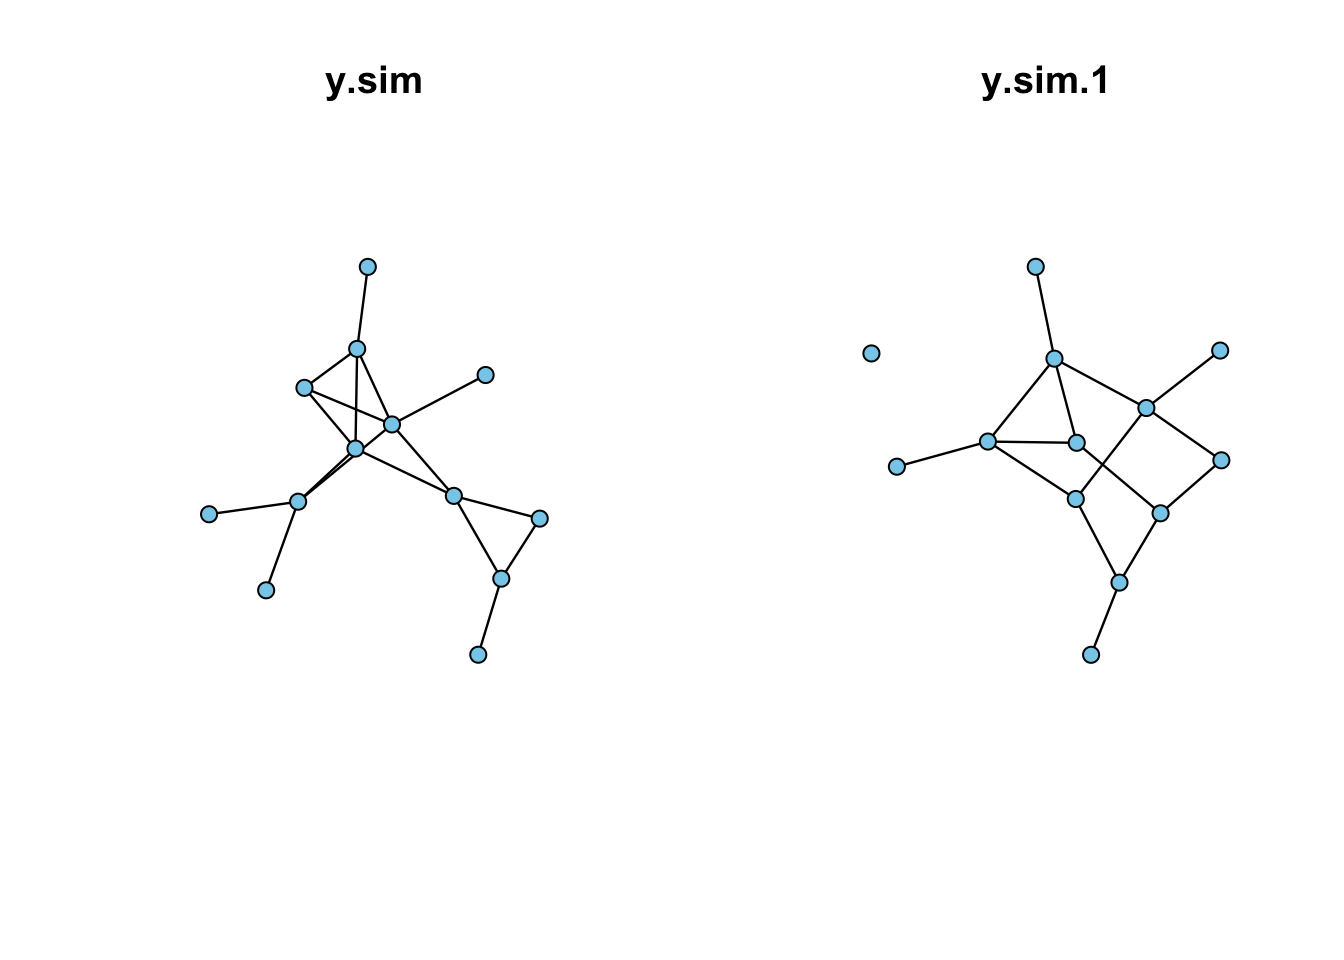
\includegraphics{SNA_BOOK_files/figure-latex/unnamed-chunk-14-1.pdf}

Now, let's simulate 50 networks from the estimated random graph model:

\begin{Shaded}
\begin{Highlighting}[]
\KeywordTok{set.seed}\NormalTok{(}\DecValTok{11}\NormalTok{)}
\NormalTok{y.sim.1_50 <-}\StringTok{ }\KeywordTok{simulate}\NormalTok{(}\KeywordTok{network}\NormalTok{(N, }\DataTypeTok{directed =} \OtherTok{FALSE}\NormalTok{) ~}\StringTok{ }\NormalTok{edges, }
                  \DataTypeTok{coef =} \NormalTok{theta$coef,}
                  \DataTypeTok{statsonly =} \OtherTok{TRUE}\NormalTok{, }\CommentTok{# returns only the values of the network statistics }
                  \DataTypeTok{nsim =} \DecValTok{50}\NormalTok{) }\CommentTok{# number of network simulated}
\KeywordTok{summary}\NormalTok{(y.sim.1_50)}
\end{Highlighting}
\end{Shaded}

\begin{verbatim}
##      edges      
##  Min.   : 5.00  
##  1st Qu.:13.25  
##  Median :15.00  
##  Mean   :14.78  
##  3rd Qu.:16.00  
##  Max.   :22.00
\end{verbatim}

\subsection{Histogram}\label{histogram}

We can plot a histogram to visualise the distribution of the number of
edges of the 50 simulated networks:

\begin{Shaded}
\begin{Highlighting}[]
\KeywordTok{hist}\NormalTok{(y.sim.1_50, }\DataTypeTok{xlab =} \StringTok{"Number of edges"}\NormalTok{, }\DataTypeTok{main =} \StringTok{""}\NormalTok{, }\DataTypeTok{col =} \StringTok{"lightgray"}\NormalTok{)}
\KeywordTok{abline}\NormalTok{(}\DataTypeTok{v =} \NormalTok{s1, }\DataTypeTok{col =} \StringTok{"red"}\NormalTok{, }\DataTypeTok{lwd =} \DecValTok{3}\NormalTok{, }\DataTypeTok{lty =} \DecValTok{2}\NormalTok{)}
\KeywordTok{abline}\NormalTok{(}\DataTypeTok{v =} \KeywordTok{mean}\NormalTok{(y.sim.1_50), }\DataTypeTok{col =} \StringTok{"blue"}\NormalTok{, }\DataTypeTok{lwd =} \DecValTok{3}\NormalTok{, }\DataTypeTok{lty =} \DecValTok{1}\NormalTok{)}
\KeywordTok{legend}\NormalTok{(}\StringTok{"topright"}\NormalTok{, }
       \KeywordTok{c}\NormalTok{(}\KeywordTok{expression}\NormalTok{(s1), }\KeywordTok{expression}\NormalTok{(}\KeywordTok{E}\NormalTok{(s[}\DecValTok{1}\NormalTok{](}\KeywordTok{tilde}\NormalTok{(y))))), }
       \DataTypeTok{lty =} \KeywordTok{c}\NormalTok{(}\DecValTok{2}\NormalTok{, }\DecValTok{1}\NormalTok{), }
       \DataTypeTok{col =} \KeywordTok{c}\NormalTok{(}\StringTok{"red"}\NormalTok{, }\StringTok{"blue"}\NormalTok{), }\DataTypeTok{lwd =} \DecValTok{3}\NormalTok{)}
\end{Highlighting}
\end{Shaded}

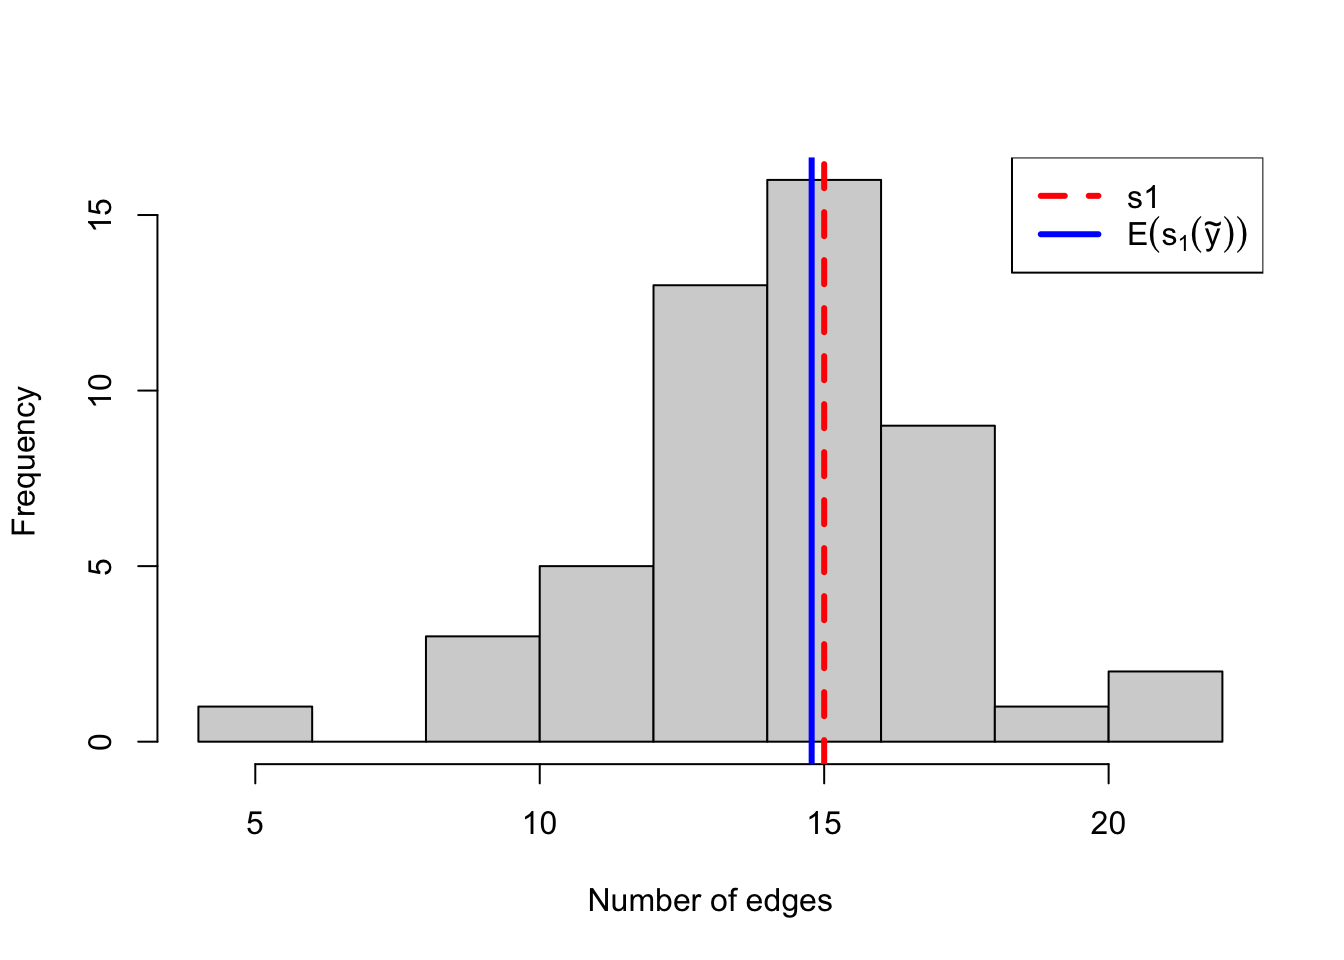
\includegraphics{SNA_BOOK_files/figure-latex/unnamed-chunk-16-1.pdf}

\subsection{Boxplot}\label{boxplot}

Alternatively, we can plot a boxplot:

\begin{Shaded}
\begin{Highlighting}[]
\KeywordTok{boxplot}\NormalTok{(y.sim.1_50, }\DataTypeTok{ylab =} \StringTok{"Number of edges"}\NormalTok{)}
\KeywordTok{points}\NormalTok{(s1, }\DataTypeTok{col =} \StringTok{"red"}\NormalTok{, }\DataTypeTok{pch =} \DecValTok{19}\NormalTok{)}
\KeywordTok{points}\NormalTok{(}\KeywordTok{mean}\NormalTok{(y.sim.1_50), }\DataTypeTok{col =} \StringTok{"blue"}\NormalTok{, }\DataTypeTok{pch =} \DecValTok{19}\NormalTok{)}
\KeywordTok{legend}\NormalTok{(}\StringTok{"topright"}\NormalTok{, }
       \KeywordTok{c}\NormalTok{(}\KeywordTok{expression}\NormalTok{(s[}\DecValTok{1}\NormalTok{](y)), }\KeywordTok{expression}\NormalTok{(}\KeywordTok{E}\NormalTok{(s[}\DecValTok{1}\NormalTok{](}\KeywordTok{tilde}\NormalTok{(y))))),}
       \DataTypeTok{pch =} \KeywordTok{c}\NormalTok{(}\DecValTok{19}\NormalTok{, }\DecValTok{19}\NormalTok{), }
       \DataTypeTok{col =} \KeywordTok{c}\NormalTok{(}\StringTok{"red"}\NormalTok{, }\StringTok{"blue"}\NormalTok{))}
\end{Highlighting}
\end{Shaded}

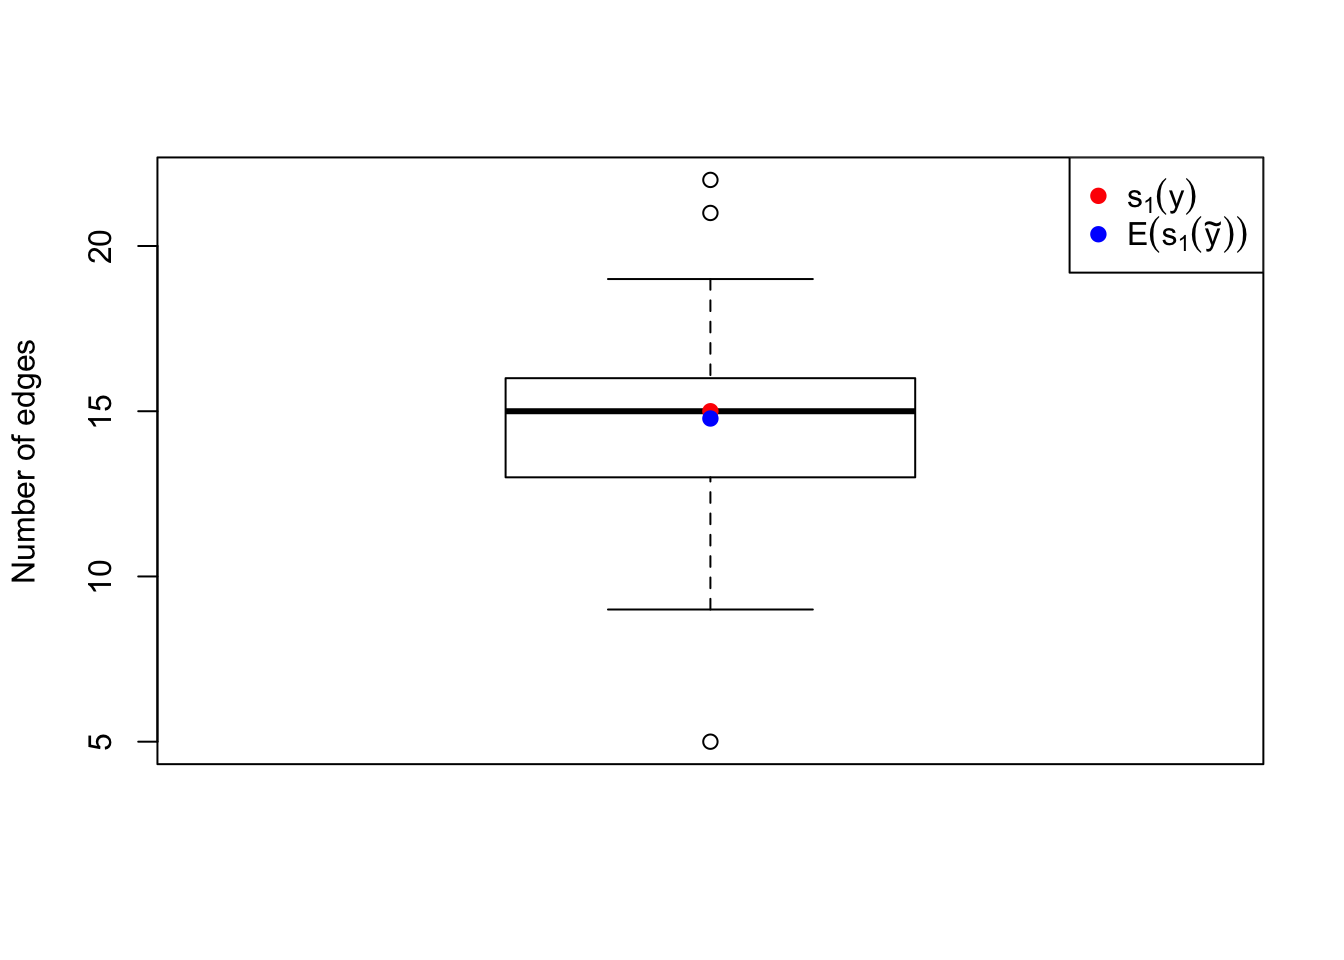
\includegraphics{SNA_BOOK_files/figure-latex/unnamed-chunk-17-1.pdf}

\section{Network statistics}\label{network-statistics}

Due to the complexity of networks, it is necessary to reduce the
information to describe essential properties of the network.

Usually this is done via \emph{network statistics} a series of counts of
sub-graph configurations, catching the relevant information.

A network statistic:

\begin{itemize}
\item
  should \textbf{describe essential properties} of the network. A
  certain property should be described in a compact and handy form. We
  would like to forget the exact structure of the underlying graph and
  concentrate on a restricted set of statistics.
\item
  should \textbf{differentiate between certain classes} of networks. A
  quite common question in network analysis regards the type of the
  measured network and how to generate models for it. This requires the
  decision about whether a generated network is similar to another one.
  In many situations, this may be done by identifying several
  statistics, which are invariant in the class of networks of interest.
\item
  may be \textbf{useful in algorithms and applications}. Some network
  statistics may be used for algorithms or calculations on the graph. Or
  they might indicate which graph elements have certain properties
  regarding the application.
\end{itemize}

\subsection{Degree distribution}\label{degree-distribution}

The degree distribution for a network consists of the values
\[\frac{D_0}{N}, \frac{D_1}{N}, \dots, \frac{D_{N-1}}{N}\] where
\(\frac{D_{k}}{N}\) equals the proportion of nodes that share edges with
exactly \(k\) other nodes.

\begin{Shaded}
\begin{Highlighting}[]
\NormalTok{Deg.dist <-}\StringTok{ }\KeywordTok{summary}\NormalTok{(y ~}\StringTok{ }\KeywordTok{degree}\NormalTok{(}\DecValTok{0}\NormalTok{:(N}\DecValTok{-1}\NormalTok{)))}
\KeywordTok{plot}\NormalTok{(Deg.dist /}\StringTok{ }\NormalTok{N, }\DataTypeTok{type =} \StringTok{"l"}\NormalTok{, }\DataTypeTok{lwd =} \DecValTok{3}\NormalTok{,}
     \DataTypeTok{xlab =} \StringTok{"Degree"}\NormalTok{,}
     \DataTypeTok{ylab =} \StringTok{"Proportion of nodes"}\NormalTok{)}
\end{Highlighting}
\end{Shaded}

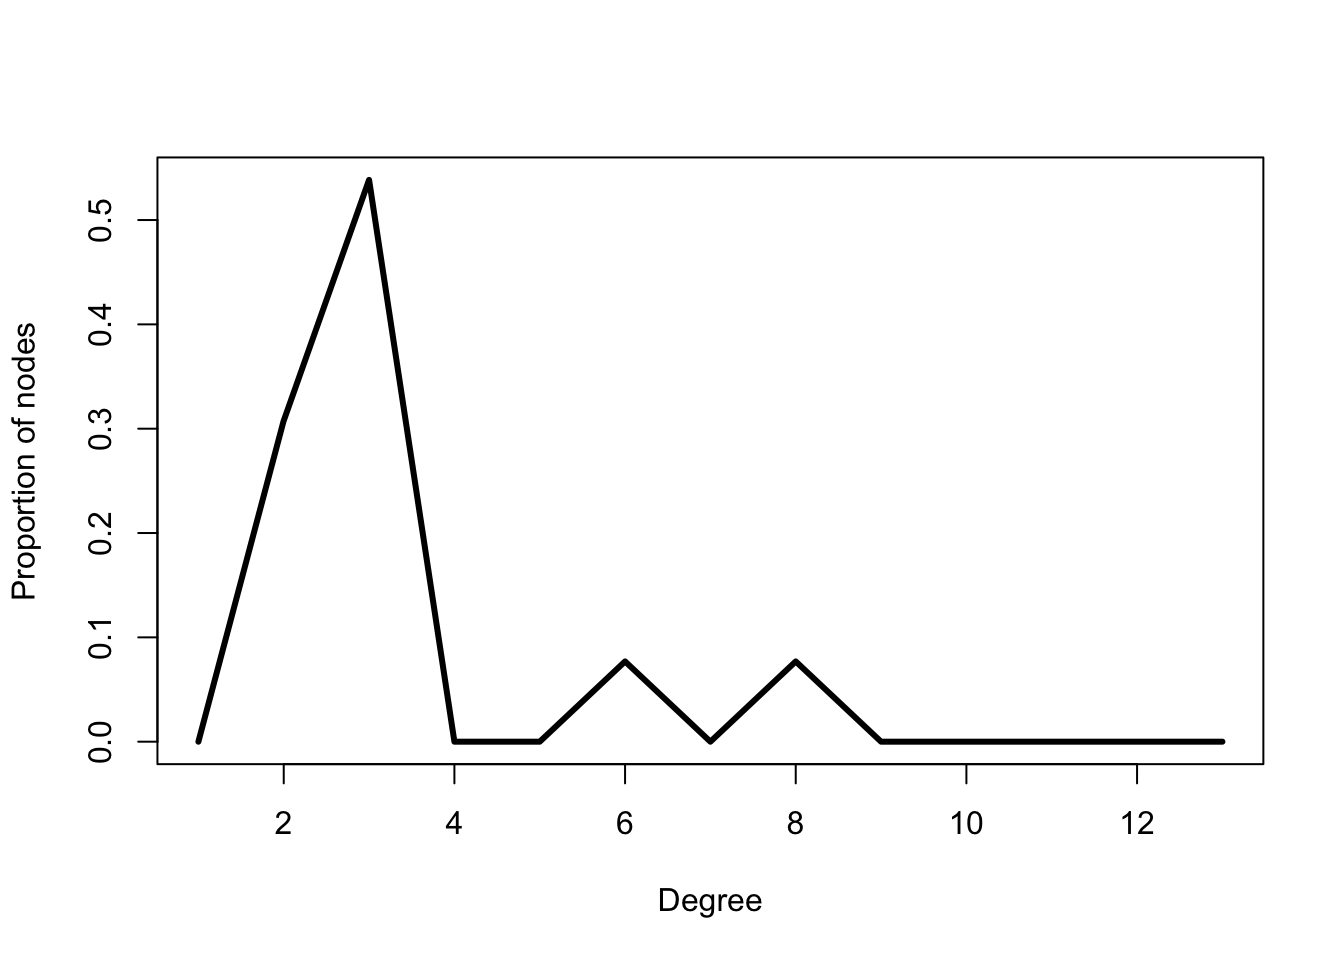
\includegraphics{SNA_BOOK_files/figure-latex/unnamed-chunk-18-1.pdf}

\subsection{Edgewise shared partners
distribution}\label{edgewise-shared-partners-distribution}

The edgewise shared partner distribution consists of the values
\[\frac{EP_0}{s_1(y)}, \frac{EP_1}{s_1(y)} \dots, \frac{EP_{N−2}}{s_1(y)}\]
where \(s_1(y)\) denotes the number of edges and \(EP_k\) equals the
number of edges whose endpoints both share edges with exactly \(k\)
other nodes.

\begin{Shaded}
\begin{Highlighting}[]
\NormalTok{Ep.dist <-}\StringTok{ }\KeywordTok{summary}\NormalTok{(y ~}\StringTok{ }\KeywordTok{esp}\NormalTok{(}\DecValTok{0}\NormalTok{:(N -}\StringTok{ }\DecValTok{1}\NormalTok{)))}
\KeywordTok{plot}\NormalTok{(Ep.dist /}\StringTok{ }\NormalTok{s1, }\DataTypeTok{type =} \StringTok{"l"}\NormalTok{, }\DataTypeTok{lwd =} \DecValTok{3}\NormalTok{,}
     \DataTypeTok{xlab =} \StringTok{"Edgewise shared partners"}\NormalTok{,}
     \DataTypeTok{ylab =} \StringTok{"Proportion of edges"}\NormalTok{)}
\end{Highlighting}
\end{Shaded}

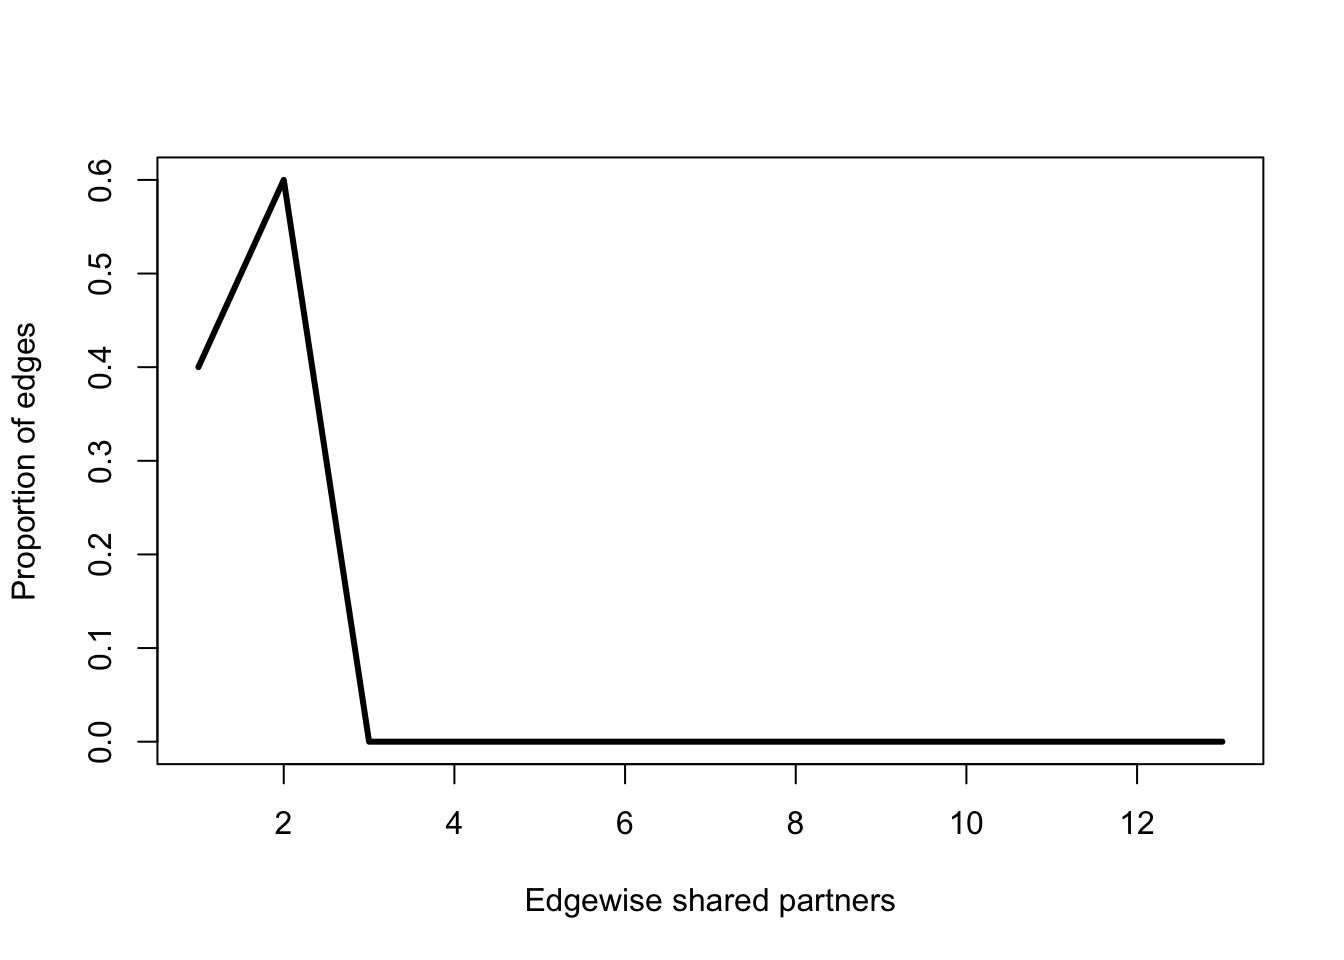
\includegraphics{SNA_BOOK_files/figure-latex/unnamed-chunk-19-1.pdf}

\subsection{Geodesic distance
distribution}\label{geodesic-distance-distribution}

The geodesic distance distribution consists of the relative frequencies
of the possible values of geodesic distance between two nodes, where the
geodesic distance between two nodes equals the length of the shortest
path joining those two nodes (or infinity if there is no such path).

For instance, because two nodes are at geodesic distance 1 if and only
if they are connected by an edge, and because there are \(\binom{N}{2}\)
possible pairs of nodes, the first value of the geodesic distance
distribution equals \(\frac{s_1(y)}{\binom{N}{2}}\). The last value, the
fraction of dyads with infinite geodesics, is also called the fraction
``unreachable'' (NR).

\begin{Shaded}
\begin{Highlighting}[]
\NormalTok{Geo.dist <-}\StringTok{ }\KeywordTok{ergm.geodistdist}\NormalTok{(y)}
\KeywordTok{plot}\NormalTok{(Geo.dist /}\StringTok{ }\NormalTok{D, }\DataTypeTok{type =} \StringTok{"l"}\NormalTok{, }\DataTypeTok{lwd =} \DecValTok{3}\NormalTok{,}
     \DataTypeTok{xlab =} \StringTok{"Minimum geodesic distance"}\NormalTok{,}
     \DataTypeTok{ylab =} \StringTok{"Proportion of dyads"}\NormalTok{)}
\end{Highlighting}
\end{Shaded}

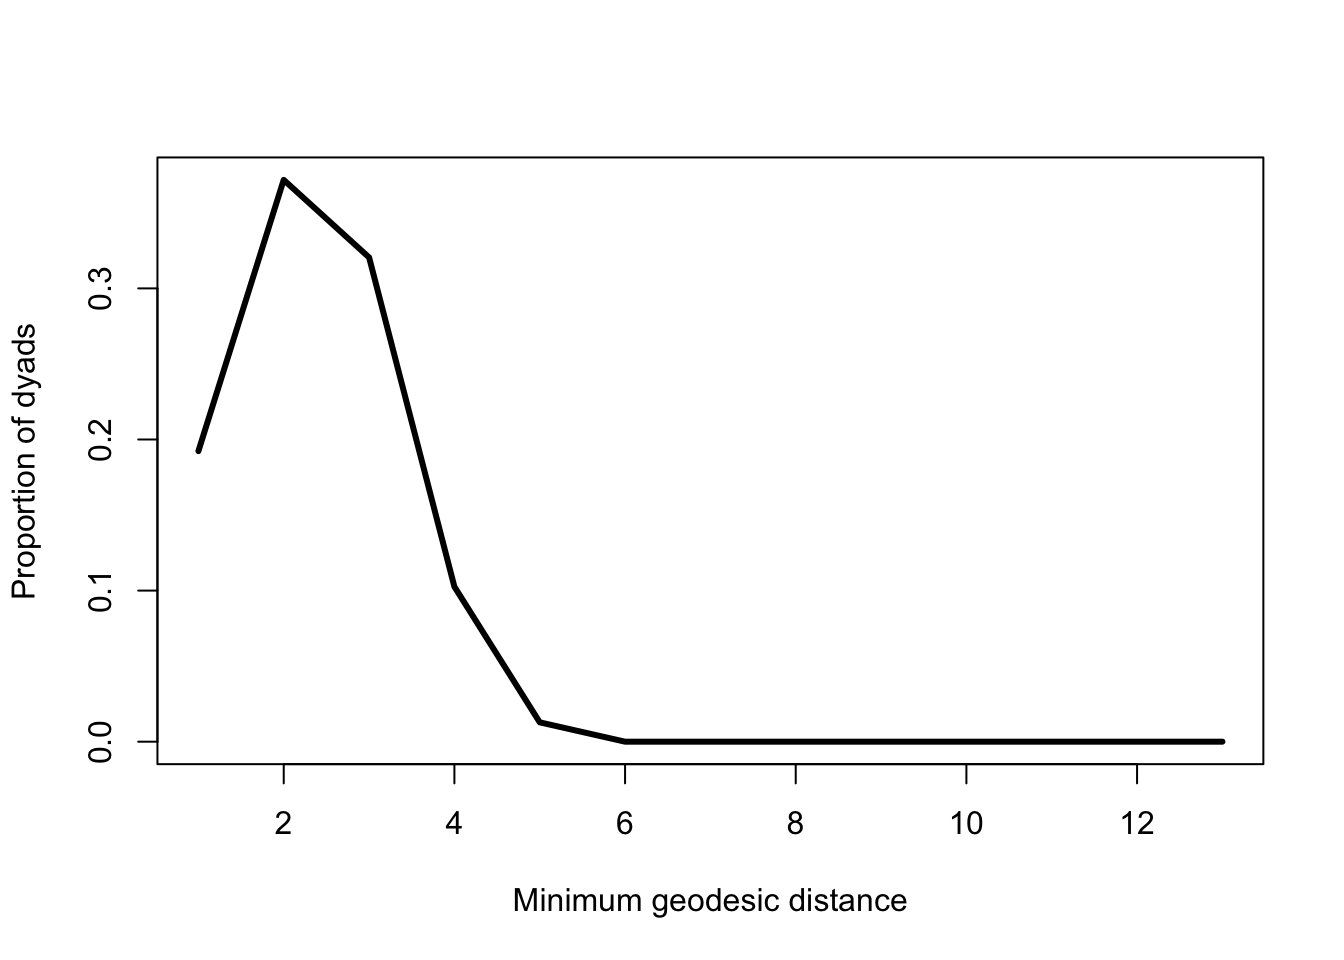
\includegraphics{SNA_BOOK_files/figure-latex/unnamed-chunk-20-1.pdf}

\section{Goodness of fit diagnostics}\label{goodness-of-fit-diagnostics}

A pragmatic way to examine the fit of the data to the estimated model
the output obtained is to implement a goodness-of-fit procedure.

To do this, a set of network graphs are simulated from the maximum
likelihood estimate of the parameter \(\hat{\theta}\) and compared to
the observed graph in terms of high-level network statistics which are
not modelled explicitly.

We can use the \texttt{gof} function:

\begin{Shaded}
\begin{Highlighting}[]
\NormalTok{gof.theta <-}\StringTok{ }\KeywordTok{gof}\NormalTok{(theta ~}\StringTok{ }\NormalTok{degree +}\StringTok{ }\NormalTok{esp +}\StringTok{ }\NormalTok{distance,}
                 \KeywordTok{control.gof.formula}\NormalTok{(}\DataTypeTok{nsim =} \DecValTok{100}\NormalTok{)) }\CommentTok{# number of simulated networks}
\end{Highlighting}
\end{Shaded}

\subsection{Graphical diagnostics}\label{graphical-diagnostics}

\begin{Shaded}
\begin{Highlighting}[]
\KeywordTok{par}\NormalTok{(}\DataTypeTok{mfrow =} \KeywordTok{c}\NormalTok{(}\DecValTok{1}\NormalTok{, }\DecValTok{3}\NormalTok{))}
\KeywordTok{plot}\NormalTok{(gof.theta, }\DataTypeTok{main =} \StringTok{''}\NormalTok{)}
\end{Highlighting}
\end{Shaded}

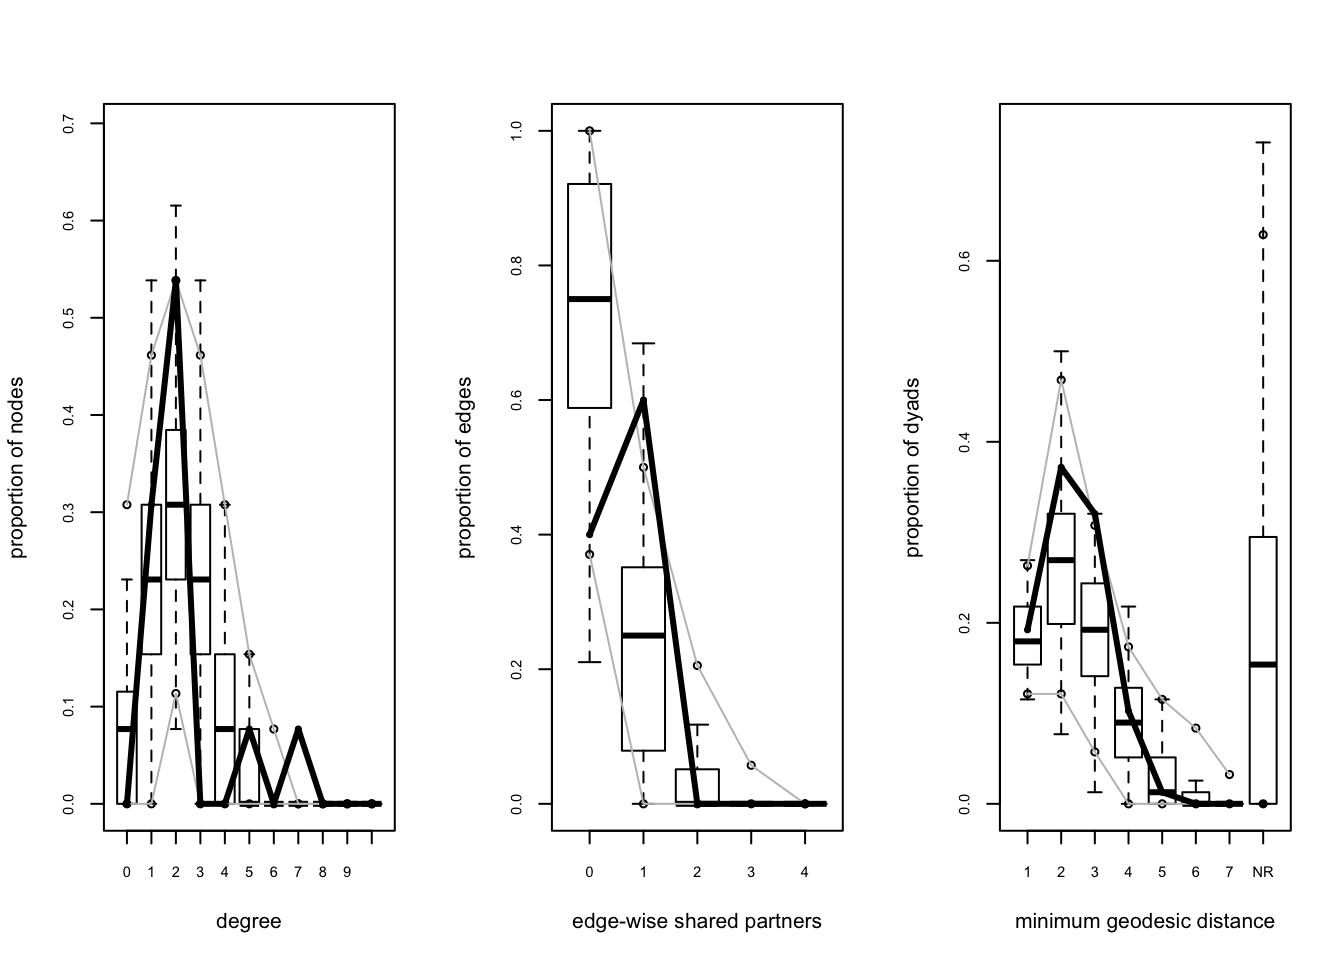
\includegraphics{SNA_BOOK_files/figure-latex/unnamed-chunk-22-1.pdf}

\subsection{Summaries}\label{summaries}

\begin{Shaded}
\begin{Highlighting}[]
\KeywordTok{summary}\NormalTok{(gof.theta)}
\end{Highlighting}
\end{Shaded}

\begin{verbatim}
## 
## Goodness-of-fit for degree 
## 
##   obs min mean max MC p-value
## 0   0   0 1.00   4       0.74
## 1   4   0 2.86   9       0.58
## 2   7   1 3.87   8       0.08
## 3   0   0 3.15   7       0.08
## 4   0   0 1.45   6       0.54
## 5   1   0 0.50   3       0.76
## 6   0   0 0.15   2       1.00
## 7   1   0 0.01   1       0.02
## 8   0   0 0.01   1       1.00
## 
## Goodness-of-fit for edgewise shared partner 
## 
##      obs min  mean max MC p-value
## esp0   6   4 10.42  18       0.12
## esp1   9   0  3.71  13       0.14
## esp2   0   0  0.50   7       1.00
## esp3   0   0  0.07   1       1.00
## 
## Goodness-of-fit for minimum geodesic distance 
## 
##     obs min  mean max MC p-value
## 1    15   9 14.70  21       0.94
## 2    29   6 21.04  39       0.32
## 3    25   1 15.19  25       0.02
## 4     8   0  6.92  17       0.90
## 5     1   0  2.40   9       1.00
## 6     0   0  0.77   8       1.00
## 7     0   0  0.16   3       1.00
## 8     0   0  0.01   1       1.00
## Inf   0   0 16.81  58       0.54
\end{verbatim}

\chapter{Exponential random graph models (ERGMs)}\label{ERGMs}

\section{Introduction}\label{introduction}

The basci assumption behind exponential random graph models (ERGMs) is
that the observed network is generated by a stochastic process in which
relational edges come into being in ways that may be shaped by the
presence or absence of other edges (and possibly node-level attributes).

In other words, the network is conceptualized as a self-organizing
system of relational edges. Substantively, the claim is that there are
local processes that generate dyadic relations, and that these processes
may depend on the surrounding social environment (i.e.~on existing
relations).

For example, we can assume that actors with similar attributes are more
likely to form friendship edges (homophily), or that if two unconnected
actors were connected to a third actor, at some point they are likely to
form a friendship tie between them (transitivity). Note that in addition
to the assumption of stochasticity, this description is also implicitly
temporal and dynamic.

\textbf{Definition} - The likelihood of an ERGM belongs to the
exponential family of distributions and represents the probability
distribution of a network graph \(y\) given a vector of parameters
\(\theta\): \[
f(y\ |\ \theta) = \frac{\exp\{\theta^T s(y)\}}{c(\theta)}.
\]

This equation states that the probability of observing a given network
graph \(y\) is equal to the exponent of the observed graph statistics
\(s(y)\) which is a function of the network data \(y\) and covariate
information \(x\) multiplied by parameter vector \(\theta\) divided by a
normalising constant term \(c(\theta)\).

\begin{Shaded}
\begin{Highlighting}[]
\KeywordTok{require}\NormalTok{(}\StringTok{'statnet'}\NormalTok{)}
\end{Highlighting}
\end{Shaded}

\section{Dependence assumptions}\label{dependence-assumptions}

Network statistics \(s(y)\) imply different assumptions regarding the
network dyadic dependence structure.

\subsection{Dyadic independence}\label{dyadic-independence}

Dyad independent network statistics imply independence between dyads:
the presence or absence of a edge does not depend the connectivity
structure of the overall network. The random graph model is a dyadic
independence model as all possible distinct edges in the network are
independent of one another: \[
Y_{ij}\ |\ \eta \sim Bernoulli(\eta),\; \forall i \ne j.
\]

\subsection{Dyadic dependence}\label{dyadic-dependence}

Dyadic dependence is an unrealistic assumption in many circumstances.

Dyad dependent network statistics imply dependence between dyads: an
edge between \(i\) and \(j\) is assumed to be dependent on other edges.

For example:

\begin{itemize}
\tightlist
\item
  \textbf{stars} statistics assume that an edge between \(i\) and \(j\)
  is contingent on any possible edge involving node \(i\) and \(j\).
\item
  \textbf{triadic} statistics assume that an edge between \(i\) and
  \(j\) is contingent on any possible edge involving any node of the
  network connected to both \(i\) and \(j\).
\end{itemize}

\section{Network statistics}\label{network-statistics-1}

Common network statistics (undirected networks):

\begin{itemize}
\item
  \emph{edge statistic}: the number of edges in the network. This
  statistic is commonly density effect
\item
  \emph{\(k\)-star statistics}: the number of \(k\)-star structures
  (where generally \(k = 2\) or \(k = 3\))
\item
  \emph{cyclic statistics}: the number of connected \(k\)-cycles (where
  generally \(k = 3 \rightarrow\) triangles)
  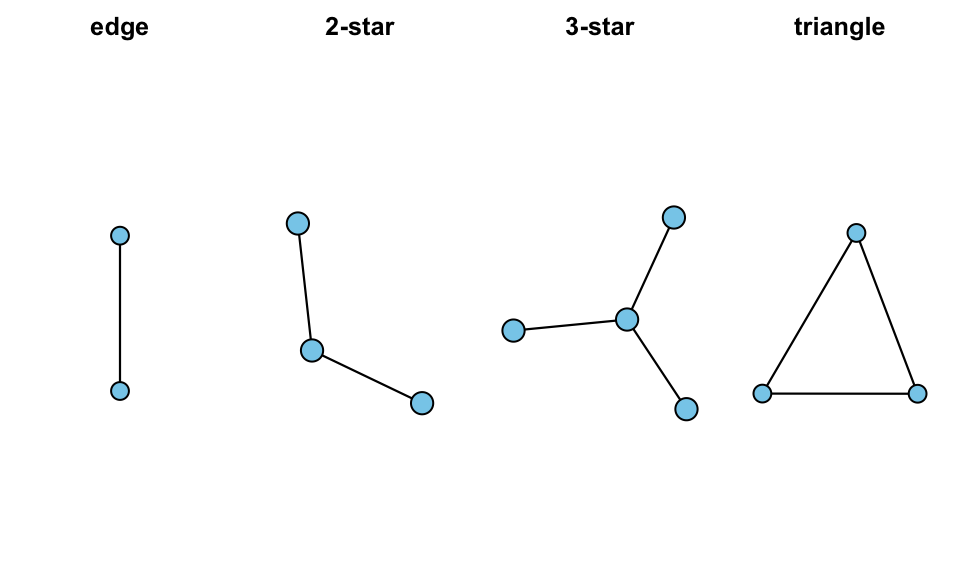
\includegraphics{SNA_BOOK_files/figure-latex/unnamed-chunk-27-1.pdf}
\end{itemize}

To get a list of network statistics implemented in the \texttt{ergm}
package:

\begin{Shaded}
\begin{Highlighting}[]
\KeywordTok{help}\NormalTok{(}\StringTok{'ergm-terms'}\NormalTok{, }\StringTok{'ergm'}\NormalTok{)}
\end{Highlighting}
\end{Shaded}

Let's consider a random 53-node undirected network:

\begin{Shaded}
\begin{Highlighting}[]
\KeywordTok{set.seed}\NormalTok{(}\DecValTok{17}\NormalTok{)}
\NormalTok{N <-}\StringTok{ }\DecValTok{53}
\NormalTok{y <-}\StringTok{ }\KeywordTok{network}\NormalTok{(N, }\DataTypeTok{directed =} \OtherTok{FALSE}\NormalTok{)}
\KeywordTok{plot}\NormalTok{(y, }\DataTypeTok{vertex.cex =} \DecValTok{2}\NormalTok{, }\DataTypeTok{vertex.col =} \StringTok{"skyblue"}\NormalTok{)}
\end{Highlighting}
\end{Shaded}

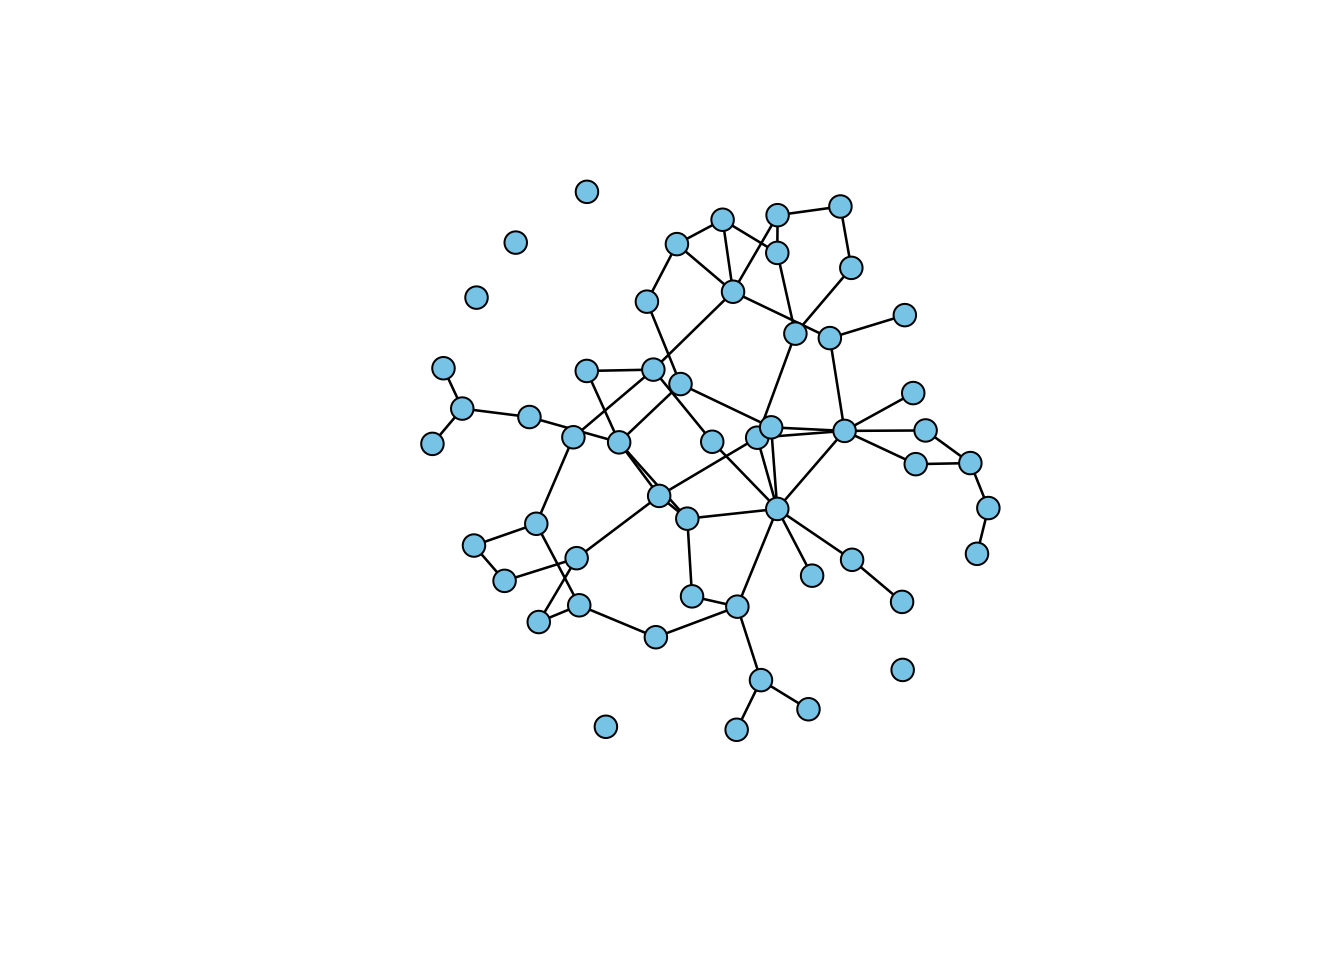
\includegraphics{SNA_BOOK_files/figure-latex/unnamed-chunk-29-1.pdf}

Let's consider an ERGM with the following network statistics:

\begin{itemize}
\tightlist
\item
  edges: \(s_1(y) = \sum_{i < j} y_{ij}\);
\item
  2-stars: \(s_2(y) = \sum_{i < j < k} y_{ij}y_{ik}\);
\item
  triangles: \(s_3(y) = \sum_{i < j < k} y_{ij}y_{ik}y_{jk}\).
\end{itemize}

The vector of observed network statistics \(s(y)\) can be calculated
using the \texttt{summary} function:

\begin{Shaded}
\begin{Highlighting}[]
\NormalTok{model}\FloatTok{.1} \NormalTok{<-}\StringTok{ }\NormalTok{y ~}\StringTok{ }\NormalTok{edges +}\StringTok{ }\KeywordTok{kstar}\NormalTok{(}\DecValTok{2}\NormalTok{) +}\StringTok{ }\NormalTok{triangle}
\KeywordTok{summary}\NormalTok{(model}\FloatTok{.1}\NormalTok{)}
\end{Highlighting}
\end{Shaded}

\begin{verbatim}
##    edges   kstar2 triangle 
##       64      157        4
\end{verbatim}

\subsection{Higher-order network
statistics}\label{higher-order-network-statistics}

Simulation-based inferential procedures have brought to light model
degeneracy problems related to ERGMs defined by traditional
specification \citep{sch11}. In order to overcome these issues, a new
specification of network statistics based on \emph{geometrically
weighted} functions of extra-triadic network statistics distributions
such as degree distributions have been proposed by
\citet{sni:pat:rob:han06}.

Some of the geometrically weighted undirected network statistics that
are common in empirical research are:

\begin{itemize}
\tightlist
\item
  \emph{Geometrically weighted degree statistic} (\texttt{gwdegree}) is
  a function of the degree counts \(D_d (y)\) defined as the number of
  nodes in \(y\) with degree \(d\):

  \begin{equation*}
  gwdegree(y, \alpha) = 
  \sum_d g_d (\alpha) D_d (y),
  \end{equation*}

  where \(g_d (y)\) is an exponential weight function defined as:

  \begin{equation*}
  g_d (\alpha) = e^{\alpha} \left\{ 1 - \left( 1 - e ^{-\alpha} \right)^{d} \right\}. 
  \end{equation*}
\end{itemize}

This statistic expresses a version of preferential attachment
\citep{alb:bar02} with edges from low degree to high degree nodes being
more probable than edges among low degree nodes.

\begin{itemize}
\tightlist
\item
  \emph{Geometrically weighted edgewise shared partner statistic}
  (\texttt{gwesp}) is a function of the edgewise shared partner
  statistics \(EP_d (y)\) defined as the number of unordered connected
  pairs \((i, j)\) (partners) that are both connected to exactly \(d\)
  other nodes:

  \begin{equation*}
  gwesp(y, \alpha) =
  \sum_d g_d (\alpha) \; EP_d (y) =
  \sum_d g_d (\alpha) \sum_{i < j} y_{ij} \mathbb{I}_{ \left\{ \sum_k y_{ik} y_{jk} = d  \right\} },
  \end{equation*}

  where \(\mathbb{I}_{\lbrace \cdot \rbrace}\) is the indicator
  function. For directed networks the geometric weighting is over
  homogeneous shared partners only (i.e., only partners on a directed
  two-path connecting the nodes in the edge and in the same direction).
\end{itemize}

This statistic provides a suitable representation of transitivity in
social networks by taking into account high-order \(k\)-triangles.

For example, let's consider the following ERGM:

\begin{Shaded}
\begin{Highlighting}[]
\NormalTok{model}\FloatTok{.2} \NormalTok{<-}\StringTok{ }\NormalTok{y ~}\StringTok{ }\NormalTok{edges +}\StringTok{ }\KeywordTok{gwesp}\NormalTok{(}\DataTypeTok{decay =} \DecValTok{1}\NormalTok{, }\DataTypeTok{fixed =} \OtherTok{TRUE}\NormalTok{)}
\KeywordTok{summary}\NormalTok{(model}\FloatTok{.2}\NormalTok{)}
\end{Highlighting}
\end{Shaded}

\begin{verbatim}
##         edges gwesp.fixed.1 
##      64.00000      11.63212
\end{verbatim}

\subsection{Statistics with nodal attributes
variables}\label{statistics-with-nodal-attributes-variables}

There are various ways of introducing node-level effects (node
attributes) into ERGMs. We assume an vector \(X\) of attribute variables
is given.

In \emph{social selection} models, attributes are assumed to be
exogenous predictors of network edges \citep{rob:ell:pat01}: edges tend
to develop between actors with certain attribute values. This means that
the interest is in the probability of the network graph \(y\) given the
observations of attributes \(x\): \(\Pr(Y = y|X = x)\).

\section{Parameter interpretation}\label{parameter-interpretation-1}

The parameter estimates associated with the network effects expressed by
the network statistics provide insights about the contribution of each
network statistic to edge formation. ERGMs allow to establish a
relationship between a binary outcome variable (presence/absence of an
edge between nodes) and a group of predictor variables (network
statistics). It models the logit-transformed probability as a linear
relationship with the predictor variables.

The conditional log-odds of an edge between \(i\) and \(j\) is: \[
\mathrm{logit} \left( \Pr(Y_{ij} = 1\ |\ Y_{-ij}, \theta ) \right) = \theta^T\ \Delta (s(y))_{ij}, 
\] where \(\Delta (s(y))_{ij}\) is the change in \(s(y)\) when the value
of \(Y_{ij}\) switch value from 0 to 1. So the coefficient \(\theta\)
can be interpreted as the log-odds of an individual edge conditional on
all others.

\section{Network simulation}\label{network-simulation-1}

The ERGM normalising constant \(c(\theta)\) is calculated over the sum
of all possible graphs on \(N\) nodes and it is therefore extremely
difficult to evaluate in presence of extra-dyadic network statistics for
all but trivially small graphs.

The simulation of graphs from the parameter values of the model can be
generally provided by MCMC algorithms. One of the convenient ways to
generate random graphs is by the Metropolis algorithm applied to an
initial adjacency matrix \(Y^{(0)}\) whose elements dyads are
stochastically updated so that at each iteration \(t\), the procedure
implies that \(Y^{(t-1)}\) and \(Y^{(t)}\) differs in only one dyad.
This mechanism cycles through the whole matrix so as to produce a
distribution \(Y^{(T)}\) tends asymptotically to the desired random
graph distribution.

In practice the algorithm compares the probability of a proposed graph
\(y'\) to the current one \(y_c\) where \(y'\) is selected at each step
by proposing a change in the current state of a single dyad \((i,j)\),
i.e.~creating a new edge or dropping an old edge and then decides
whether or not accept the proposed network with the following acceptance
probability:

\begin{equation*}
\alpha 
   =\min
    \left\lbrace 
    1,\frac{p(y'\ |\ \theta_0)\ q(y_c \rightarrow y')}
           {p(y_c\ |\ \theta_0)\ q(y' \rightarrow y_c)}
    \right\rbrace 
   =\exp
    \left\lbrace 
    \theta_0^t 
    \left[
    s(y') - s(y_c)
    \right]
    \right\rbrace
\end{equation*}

where \(q(y_c \rightarrow y')\) and \(q(y' \rightarrow y_c)\) denote the
probability of \(y'\) given \(y_c\) and of \(y_c\) given \(y'\)
respectively.

The behaviour of MCMC algorithm is dependent on the choice of the
proposal density \(q(\cdot)\) and on the network statistics \(s(\cdot)\)
although it is proven that in principle the Metropolis yields
convergence to the target distribution.

Suppose we want to simulate undirected networks on 53 nodes from the
same ERGM defined above with parameter values:

\begin{itemize}
\tightlist
\item
  \(\theta_1 = -1.9\), parameter related to the edge statistic
  \(s_1(y)\);
\item
  \(\theta_2 = -0.1\), parameter related to the 2-star statistic
  \(s_2(y)\);
\item
  \(\theta_3 = 0.4\), parameter related to the triangle statistics
  \(s_3(y)\).
\end{itemize}

We can use the \texttt{simulate} function to do that:

\begin{Shaded}
\begin{Highlighting}[]
\KeywordTok{set.seed}\NormalTok{(}\DecValTok{11}\NormalTok{)}
\NormalTok{y.sim <-}\StringTok{ }\KeywordTok{simulate}\NormalTok{(}\KeywordTok{network}\NormalTok{(N, }\DataTypeTok{directed =} \OtherTok{FALSE}\NormalTok{) ~}\StringTok{ }\NormalTok{edges +}\StringTok{ }\KeywordTok{kstar}\NormalTok{(}\DecValTok{2}\NormalTok{) +}\StringTok{ }\NormalTok{triangle, }
                  \DataTypeTok{coef =} \KeywordTok{c}\NormalTok{(-}\FloatTok{1.9}\NormalTok{, -}\FloatTok{0.1}\NormalTok{, }\FloatTok{0.4}\NormalTok{),}
                  \DataTypeTok{statsonly =} \OtherTok{TRUE}\NormalTok{,}
                  \DataTypeTok{nsim =} \DecValTok{1000}\NormalTok{,}
                  \DataTypeTok{control =} \KeywordTok{control.simulate.formula}\NormalTok{(}\DataTypeTok{MCMC.burnin =} \DecValTok{1000}\NormalTok{,   }\CommentTok{# burnin }
                                                     \DataTypeTok{MCMC.interval =} \DecValTok{100}\NormalTok{)) }\CommentTok{# mcmc thinning interval }
\KeywordTok{summary}\NormalTok{(y.sim)}
\end{Highlighting}
\end{Shaded}

\begin{verbatim}
##      edges         kstar2         triangle    
##  Min.   : 78   Min.   :214.0   Min.   : 0.00  
##  1st Qu.: 97   1st Qu.:326.8   1st Qu.: 8.00  
##  Median :102   Median :365.0   Median :11.00  
##  Mean   :102   Mean   :367.1   Mean   :11.18  
##  3rd Qu.:107   3rd Qu.:405.0   3rd Qu.:14.00  
##  Max.   :126   Max.   :597.0   Max.   :31.00
\end{verbatim}

We can analyse the MCMC output diagnostics using the \texttt{coda}
package:

\begin{Shaded}
\begin{Highlighting}[]
\KeywordTok{require}\NormalTok{(coda)}
\end{Highlighting}
\end{Shaded}

\subsection{Trace and density plots}\label{trace-and-density-plots}

\begin{Shaded}
\begin{Highlighting}[]
\KeywordTok{plot}\NormalTok{(}\KeywordTok{mcmc}\NormalTok{(y.sim))}
\end{Highlighting}
\end{Shaded}

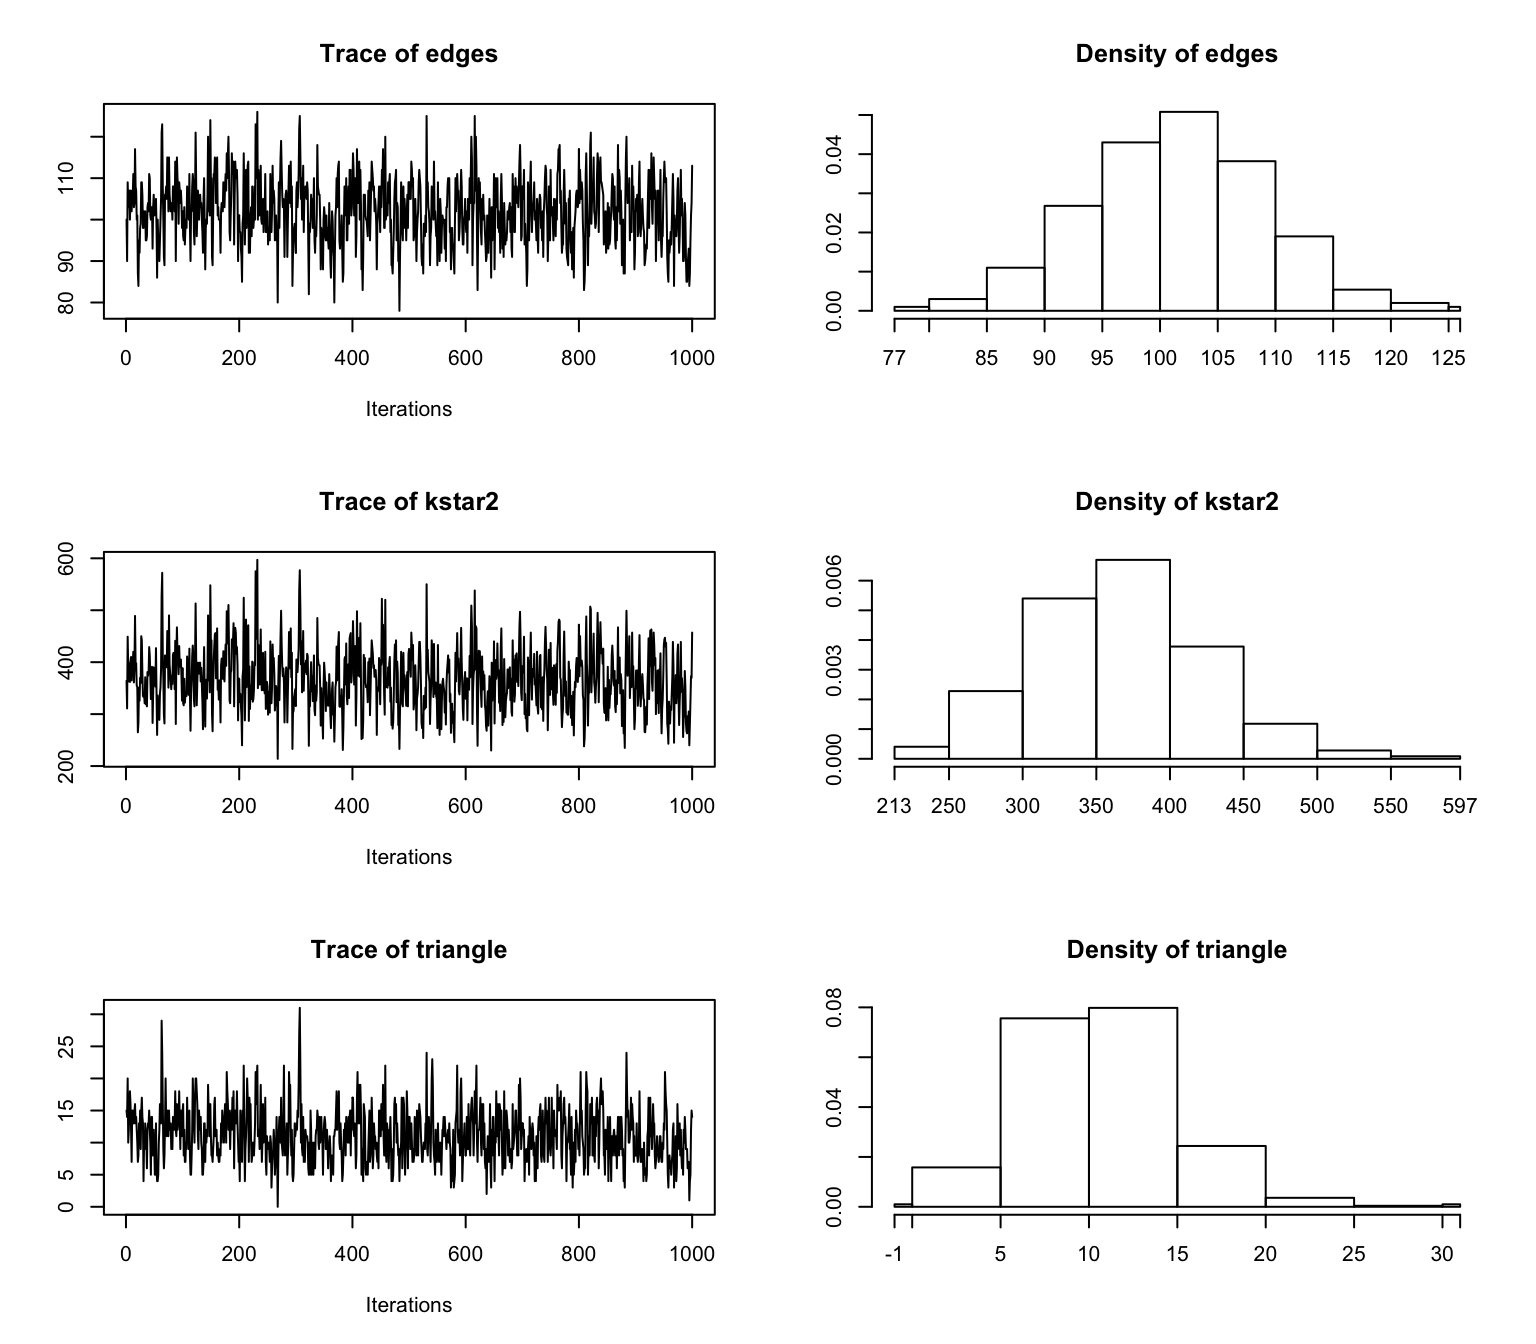
\includegraphics{SNA_BOOK_files/figure-latex/unnamed-chunk-34-1.pdf}

\subsection{Auto-correlation plots}\label{auto-correlation-plots}

\begin{Shaded}
\begin{Highlighting}[]
\KeywordTok{acfplot}\NormalTok{(}\KeywordTok{mcmc}\NormalTok{(y.sim))}
\end{Highlighting}
\end{Shaded}

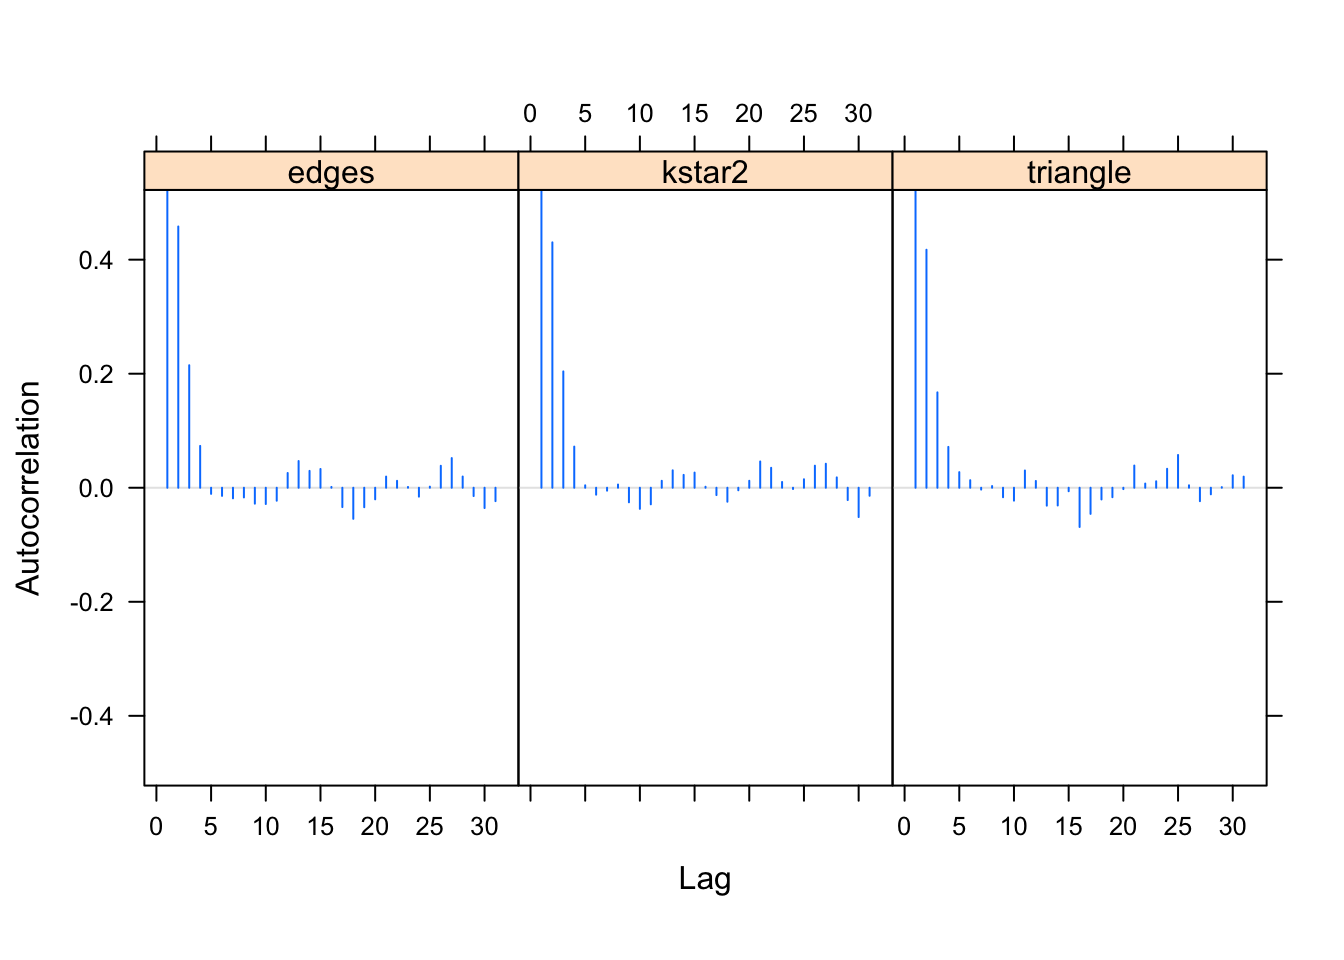
\includegraphics{SNA_BOOK_files/figure-latex/unnamed-chunk-35-1.pdf}

\chapter{Maximum likelihood estimation for ERGMs}\label{MLE_ERGMs}

The estimation procedure starts assuming that the observed network \(y\)
is just one realization of a set of many possible networks that could
have been formed by the same underlying structural processes. Each
network statistic \(s(y)\) is conceptualised as having a particular
probability of occurring which is incorporated into the model as a
parameter vector \(\theta\).

The aim of the estimation is to find accurately a parameter value so
that the observed network has the highest possible likelihood of being
simulated by the given model. In other words, when attempting to
generate an ERGM we find the set of parameters which maximise the
probability that any random network graph generated by simulating from
the ERGM will be identical to the observed network in terms of network
statistics:

\begin{equation*}
\mathbb{E}_{y\ |\ \theta}\left[s(y)\right] = s(y)
\end{equation*}

where \(\mathbb{E}_{y\ |\ \theta}\) is the expectation under the
likelihood distribution \(p(y\ |\ \theta)\) so that it ensures that the
probability mass of the ERGM is centred at \(s(y)\).

In practice, an exact solution for the ERGM is actually impossible to
calculate directly due to the \textbf{intractability} of the normalising
constant \(c(\theta)\).

\section{Monte Carlo maximum likelihood estimation
(MC-MLE)}\label{monte-carlo-maximum-likelihood-estimation-mc-mle}

The most advanced classical estimation method used is the Monte Carlo
Maximum Likelihood Estimation (MC-MLE) procedure proposed by
\href{http://www.jstor.org/stable/2345852}{Geyer and Thompson (1992)}.

This involves the simulation of a set of random networks from a starting
set of estimated parameter values \(\theta_0\), and then the progressive
refinement (until convergence) of the parameter values by measuring how
closely these networks match the observed network.

Let's denote with \(q_{\theta}(y) = \exp\{ \theta^t s(y) \}\) the
unnormalised likelihood. Mathematically, the key identity of the MC-MLE
method is the following:

\begin{align}
\frac {c(\theta)} {c(\theta_0)} 
= \mathbb{E}_{y\ |\ \theta_0} 
\left[ 
\frac {q_{\theta}(y)} {q_{\theta_0}(y)} 
\right] 
&= \sum_{y} 
\frac {q_{\theta}(y)} {q_{\theta_0}(y)} 
\frac {q_{\theta_0}(y)} {z(\theta_0)} \label{eqn:key}
\\
&\approx \frac{1}{m}\sum_{i=1}^m \exp\left\{ (\theta-\theta_0)^t s(y_i) \right\}\notag
\end{align}

where \(q(\cdot)\) is the unnormalised likelihood, \(\theta_0\) is fixed
set of parameter values, and \(\mathbb{E}_{y\ |\ \theta_0}\) denotes an
expectation taken with respect to the distribution
\(p(y\ |\ \theta_0)\). In practice this ratio of normalising constants
is approximated using graphs \(y_1,\dots,y_m\) sampled via MCMC from
\(p(y\ |\ \theta_0)\) and importance sampling.

This yields the following approximated log likelihood ratio:

\begin{equation} 
w_{\theta_0}(\theta)=\ell(\theta)-\ell(\theta_0) \approx (\theta - \theta_0)^t s(y) - 
\log\left[ \frac{1}{m}\sum_{i=1}^m \exp\left\{ (\theta-\theta_0)^t s(y_i) \right\} \right] 
\label{eqn:gey:thom}
\end{equation}

where \(\ell(\cdot)\) is the log-likelihood. \(w_{\theta_0}\) is a
function of \(\theta\), and its maximum value serves as a Monte Carlo
estimate of the MLE.

A crucial aspect of this algorithm is the choice of \(\theta_0\).
Ideally \(\theta_0\) should be very close to the maximum likelihood
estimator of \(\theta\). Viewed as a function of \(\theta\),
\(w_{\theta_0}(\theta)\) is very sensitive to the choice of
\(\theta_0\). A poorly chosen value of \(\theta_0\) may lead to an
objective function that cannot even be maximised.

The result of the MC-MLE procedure is a set of estimated parameter
values and relative standard errors which measure the degree of accuracy
and significance of the estimates.

To implement the MC-MLE procedure we can use the \texttt{ergm} function:

\begin{Shaded}
\begin{Highlighting}[]
\KeywordTok{set.seed}\NormalTok{(}\DecValTok{11}\NormalTok{)}
\NormalTok{model}\FloatTok{.2} \NormalTok{<-}\StringTok{ }\NormalTok{y ~}\StringTok{ }\NormalTok{edges +}\StringTok{ }
\StringTok{               }\KeywordTok{gwesp}\NormalTok{(}\DataTypeTok{decay =} \DecValTok{1}\NormalTok{, }\DataTypeTok{fixed =} \OtherTok{TRUE}\NormalTok{) +}\StringTok{ }
\StringTok{               }\KeywordTok{gwnsp}\NormalTok{(}\DataTypeTok{decay =} \DecValTok{1}\NormalTok{, }\DataTypeTok{fixed =} \OtherTok{TRUE}\NormalTok{)}
\NormalTok{MLE}\FloatTok{.2} \NormalTok{<-}\StringTok{ }\KeywordTok{ergm}\NormalTok{(model}\FloatTok{.2}\NormalTok{)}
\end{Highlighting}
\end{Shaded}

\begin{verbatim}
## Starting maximum likelihood estimation via MCMLE:
## Iteration 1 of at most 20: 
## The log-likelihood improved by 0.004112 
## Step length converged once. Increasing MCMC sample size.
## Iteration 2 of at most 20: 
## The log-likelihood improved by 0.0082 
## Step length converged twice. Stopping.
## Evaluating log-likelihood at the estimate. Using 20 bridges: 1 2 3 4 5 6 7 8 9 10 11 12 13 14 15 16 17 18 19 20 .
## 
## This model was fit using MCMC.  To examine model diagnostics and check for degeneracy, use the mcmc.diagnostics() function.
\end{verbatim}

\begin{Shaded}
\begin{Highlighting}[]
\KeywordTok{summary}\NormalTok{(MLE}\FloatTok{.2}\NormalTok{)}
\end{Highlighting}
\end{Shaded}

\begin{verbatim}
## 
## ==========================
## Summary of model fit
## ==========================
## 
## Formula:   y ~ edges + gwesp(decay = 1, fixed = TRUE) + gwnsp(decay = 1, 
##     fixed = TRUE)
## 
## Iterations:  2 out of 20 
## 
## Monte Carlo MLE Results:
##                Estimate Std. Error MCMC % p-value    
## edges         -3.126974   0.414423      0  <1e-04 ***
## gwesp.fixed.1  0.194962   0.179318      0   0.277    
## gwnsp.fixed.1  0.004851   0.089213      0   0.957    
## ---
## Signif. codes:  0 '***' 0.001 '**' 0.01 '*' 0.05 '.' 0.1 ' ' 1
## 
##      Null Deviance: 1910  on 1378  degrees of freedom
##  Residual Deviance:  517  on 1375  degrees of freedom
##  
## AIC: 523    BIC: 538.6    (Smaller is better.)
\end{verbatim}

\begin{Shaded}
\begin{Highlighting}[]
\KeywordTok{mcmc.diagnostics}\NormalTok{(MLE}\FloatTok{.2}\NormalTok{)}
\end{Highlighting}
\end{Shaded}

\begin{verbatim}
## Sample statistics summary:
## 
## Iterations = 16384:4209664
## Thinning interval = 1024 
## Number of chains = 1 
## Sample size per chain = 4096 
## 
## 1. Empirical mean and standard deviation for each variable,
##    plus standard error of the mean:
## 
##                 Mean     SD Naive SE Time-series SE
## edges         1.0830  8.514   0.1330         0.1265
## gwesp.fixed.1 0.5493  7.271   0.1136         0.1136
## gwnsp.fixed.1 4.4974 38.127   0.5957         0.5957
## 
## 2. Quantiles for each variable:
## 
##                 2.5%     25%       50%    75% 97.5%
## edges         -15.00  -5.000 1.000e+00  7.000 18.00
## gwesp.fixed.1 -11.63  -5.632 3.451e-13  5.264 17.26
## gwnsp.fixed.1 -60.49 -22.240 8.964e-01 28.528 85.71
## 
## 
## Sample statistics cross-correlations:
##                   edges gwesp.fixed.1 gwnsp.fixed.1
## edges         1.0000000     0.6410327     0.9557442
## gwesp.fixed.1 0.6410327     1.0000000     0.6050813
## gwnsp.fixed.1 0.9557442     0.6050813     1.0000000
## 
## Sample statistics auto-correlation:
## Chain 1 
##                 edges gwesp.fixed.1 gwnsp.fixed.1
## Lag 0     1.000000000   1.000000000  1.000000e+00
## Lag 1024  0.003546387   0.020586964  3.443736e-05
## Lag 2048 -0.021609688  -0.007190510 -2.622667e-02
## Lag 3072 -0.032834876   0.007026375 -2.331004e-02
## Lag 4096 -0.013443575  -0.009443708 -1.369215e-02
## Lag 5120  0.008690002  -0.010584478  1.835021e-02
## 
## Sample statistics burn-in diagnostic (Geweke):
## Chain 1 
## 
## Fraction in 1st window = 0.1
## Fraction in 2nd window = 0.5 
## 
##         edges gwesp.fixed.1 gwnsp.fixed.1 
##       -1.7545       -0.9937       -2.2127 
## 
## Individual P-values (lower = worse):
##         edges gwesp.fixed.1 gwnsp.fixed.1 
##    0.07934137    0.32037506    0.02691517 
## Joint P-value (lower = worse):  0.1506554 .
\end{verbatim}

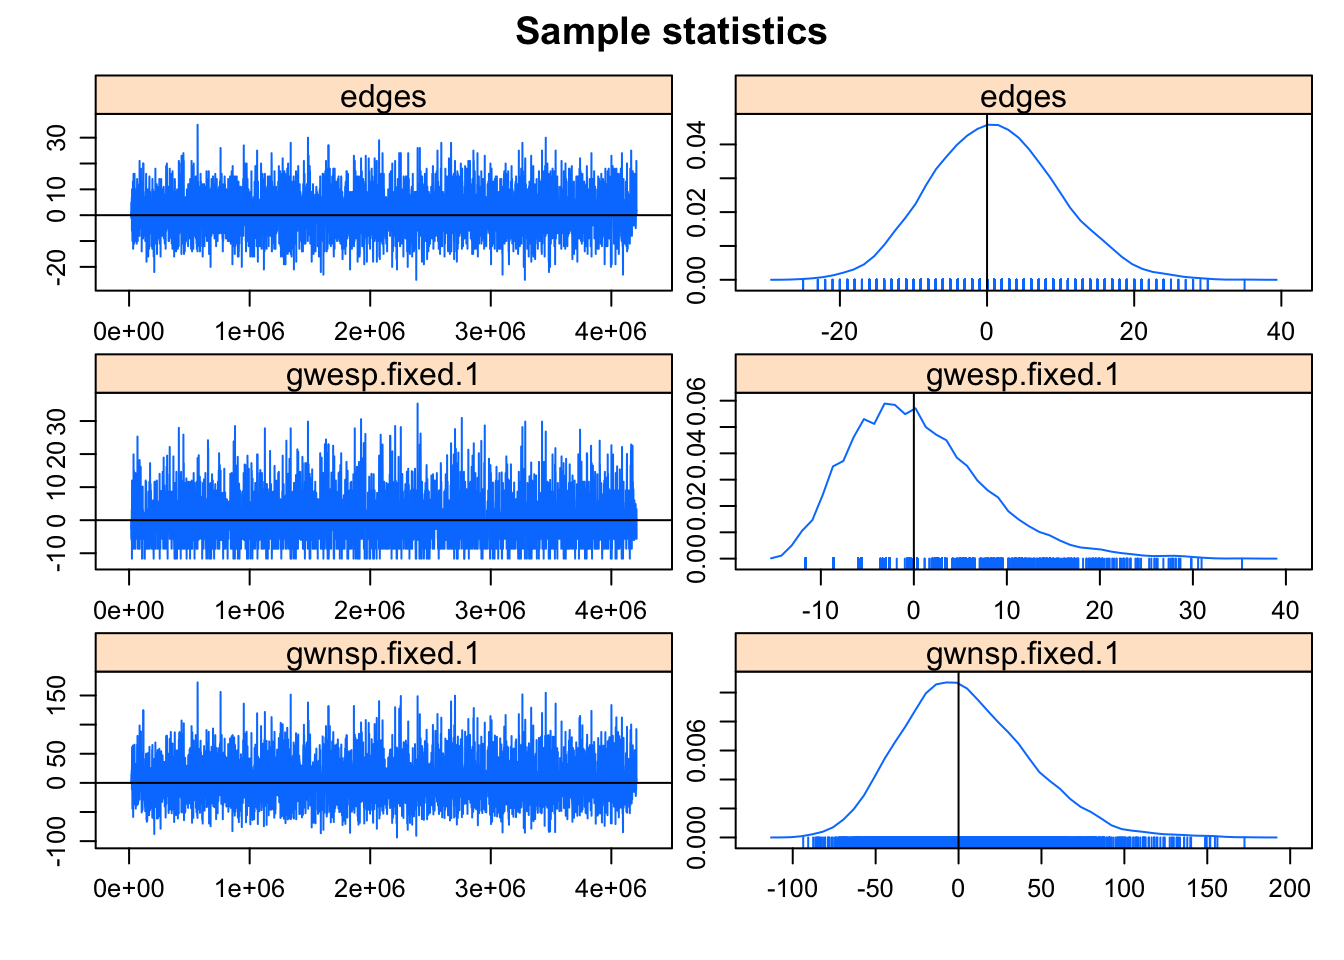
\includegraphics{SNA_BOOK_files/figure-latex/unnamed-chunk-37-1.pdf}

\begin{verbatim}
## 
## MCMC diagnostics shown here are from the last round of simulation, prior to computation of final parameter estimates. Because the final estimates are refinements of those used for this simulation run, these diagnostics may understate model performance. To directly assess the performance of the final model on in-model statistics, please use the GOF command: gof(ergmFitObject, GOF=~model).
\end{verbatim}

\section{Goodness of fit
diagnostics}\label{goodness-of-fit-diagnostics-1}

If the estimated ERGM is a good fit to the observed data, then networks
simulated \(y_1, \dots, y_m\) from its MLE should resemble the
connectivity structure of the observed data \(y\).

To do this, \(m = 100\) graphs are simulated from the maximum likelihood
estimate of the parameter vector \(\hat{\theta}\) and compared to the
observed graph in terms of high-level network statistics which are not
modelled explicitly:

\begin{Shaded}
\begin{Highlighting}[]
\NormalTok{model}\FloatTok{.2}\NormalTok{.gof <-}\StringTok{ }\KeywordTok{gof}\NormalTok{(MLE}\FloatTok{.2} \NormalTok{~}\StringTok{ }\NormalTok{degree +}\StringTok{ }\NormalTok{esp +}\StringTok{ }\NormalTok{distance,}
                   \KeywordTok{control.gof.formula}\NormalTok{(}\DataTypeTok{nsim =} \DecValTok{100}\NormalTok{))}
\end{Highlighting}
\end{Shaded}

\subsection{Graphical diagnostics}\label{graphical-diagnostics-1}

\begin{Shaded}
\begin{Highlighting}[]
\KeywordTok{par}\NormalTok{(}\DataTypeTok{mfrow =} \KeywordTok{c}\NormalTok{(}\DecValTok{1}\NormalTok{, }\DecValTok{3}\NormalTok{))}
\KeywordTok{plot}\NormalTok{(model}\FloatTok{.2}\NormalTok{.gof, }\DataTypeTok{main =} \StringTok{''}\NormalTok{)}
\end{Highlighting}
\end{Shaded}

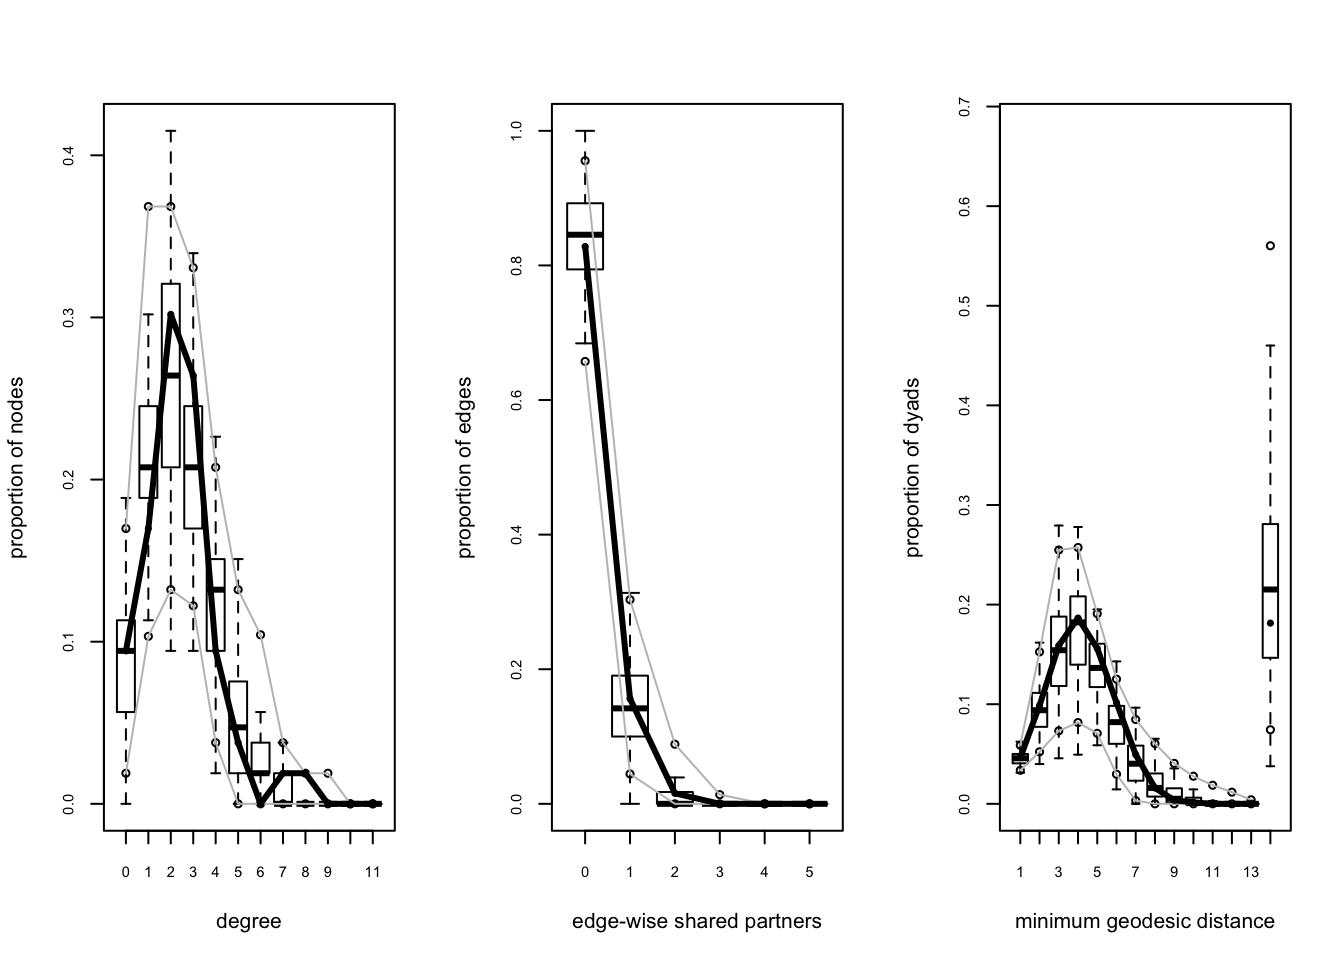
\includegraphics{SNA_BOOK_files/figure-latex/unnamed-chunk-39-1.pdf}

\subsection{Summaries}\label{summaries-1}

\begin{Shaded}
\begin{Highlighting}[]
\KeywordTok{summary}\NormalTok{(model}\FloatTok{.2}\NormalTok{.gof)}
\end{Highlighting}
\end{Shaded}

\begin{verbatim}
## 
## Goodness-of-fit for degree 
## 
##    obs min  mean max MC p-value
## 0    5   0  4.79  10       1.00
## 1    9   4 11.80  22       0.42
## 2   16   5 14.10  22       0.72
## 3   14   5 10.95  20       0.36
## 4    5   1  6.46  12       0.70
## 5    2   0  2.68  10       1.00
## 6    0   0  1.53   7       0.44
## 7    1   0  0.48   2       0.74
## 8    1   0  0.13   2       0.22
## 9    0   0  0.07   1       1.00
## 10   0   0  0.01   1       1.00
## 
## Goodness-of-fit for edgewise shared partner 
## 
##      obs min  mean max MC p-value
## esp0  53  35 52.57  76       0.96
## esp1  10   0  9.61  29       0.82
## esp2   1   0  0.97   8       0.86
## esp3   0   0  0.05   1       1.00
## 
## Goodness-of-fit for minimum geodesic distance 
## 
##     obs min   mean max MC p-value
## 1    64  43  63.20  86       0.96
## 2   136  55 132.85 234       0.88
## 3   219  63 213.89 385       0.86
## 4   257  68 239.57 383       0.90
## 5   215  59 185.51 269       0.58
## 6   140  20 109.02 197       0.42
## 7    68   0  57.13 133       0.72
## 8    22   0  28.33 109       1.00
## 9     5   0  14.27  86       0.92
## 10    2   0   6.77  68       0.92
## 11    0   0   3.15  44       1.00
## 12    0   0   1.38  22       1.00
## 13    0   0   0.40   9       1.00
## 14    0   0   0.06   2       1.00
## Inf 250  52 322.47 931       0.84
\end{verbatim}

\chapter{Bayesian inference for ERGMs}\label{Bayes_ERGMs}

\section{Parameter inference via approximate exchange
algorithm}\label{parameter-inference-via-approximate-exchange-algorithm}

Bayesian inference for ERGMs is based on the posterior distribution of
\(\theta\) given the data \(y\): \[
p(\theta | y) 
= p(y | \theta)\; \frac{p(\theta)}{p(y)} 
= \frac{ \exp \{ \theta^t s(y)\} }
       {z(\theta)}\; \frac{p(\theta)}{p(y)},
\] where \(p(\theta)\) is the prior parameter distribution and \(p(y)\)
is the evidence or marginal likelihood of \(y\) which is typically
intractable.

Standard MCMC methods such as the Metropolis-Hastings algorithm, can
deal with posterior estimation as long as the target posterior density
is known up to the model evidence \(p(y)\). Unfortunately in the ERGM
context the posterior density \(p(\theta | y)\) of non-trivially small
ERGMs includes two intractable normalising constants, the model evidence
\(p(y)\) and \(z(\theta)\). For this reason, the ERGM posterior density
is \textbf{doubly intractable}.

In order to carry out Bayesian inference for ERGMs, the \texttt{Bergm}
package makes use of MCMC techniques \citep{cai:fri11}. The
\emph{approximate exchange algorithm} circumvents the problem of
computing the normalising constants of the ERGM likelihoods, while the
use of multiple chains and efficient adaptive proposal strategies are
able to speed up the computations and improve chain mixing quite
significantly.

Let's denote \(q_{\theta}(y) = \exp \{ \theta^t s(y) \}\) the
unnormalised likelihood. The approximate exchange algorithm implemented
by the \texttt{bergm} function can be summarised in the following way:

\begin{enumerate}
\def\labelenumi{\arabic{enumi}.}
\tightlist
\item
  Gibbs update of \((\theta',y')\)
\end{enumerate}

\(\qquad\)i) Draw \(\theta' \sim h(\cdot|\theta)\)

\begin{enumerate}
\def\labelenumi{\roman{enumi})}
\setcounter{enumi}{1}
\tightlist
\item
  Approximately draw \(y' \sim f(\cdot|\theta')\) via MCMC
\end{enumerate}

\begin{enumerate}
\def\labelenumi{\arabic{enumi}.}
\setcounter{enumi}{1}
\tightlist
\item
  Accept move from \(\theta\) to \(\theta'\) with probability: \[
          1 \wedge \frac{q_{\theta'}(y)}{q_{\theta}(y)}
          \frac{p(\theta')}{p(\theta)} 
          \frac{h(\theta|\theta')}{h(\theta'|\theta)}
          \frac{q_{\theta}(y')}{q_{\theta'}(y')} 
          \times \underbrace{\frac{z(\theta)z(\theta')}{z(\theta')z(\theta)}}_{1}.
          \]
\end{enumerate}

\subsection{Parallel adaptive direction
sampler}\label{parallel-adaptive-direction-sampler}

In order to improve mixing a parallel adaptive direction sampler (ADS)
\citep{gil:rob:geo94, rob:gil94} is considered: at the \(i\)-th
iteration of the algorithm we have a collection of \(H\) different
chains interacting with one another. By construction, the state space
consists of \(\{\theta_1,\dots,\theta_H\}\) with target distribution
\(p(\theta_1|y)\otimes\dots\otimes p(\theta_H | y)\). A parallel ADS
move consists of generating a new value \(\theta'_h\) from the
difference of two parameters \(\theta_{h_1}\) and \(\theta_{h_2}\)
(randomly selected from other chains) multiplied by a scalar term
\(\gamma\) which is called parallel ADS move factor plus a random term
\(\epsilon\) called parallel ADS move parameter.

Consider the Zachary Karate club social network consisting of social
relations in a university karate club involving 34 individuals. The
nodal covariate \texttt{faction.id} is encoding the faction alignment
coded numerically, as -2 (strongly Mr.~Hi's), -1 (weakly Mr.~Hi's), 0
(neutral), +1 (weakly John's), and +2 (strongly John's):

\begin{Shaded}
\begin{Highlighting}[]
\KeywordTok{library}\NormalTok{(Bergm); }\KeywordTok{library}\NormalTok{(statnet)}
\KeywordTok{data}\NormalTok{(zach)}
\NormalTok{y <-}\StringTok{ }\NormalTok{zach}
\NormalTok{y.node.col <-}\StringTok{ }\KeywordTok{rainbow}\NormalTok{(}\DecValTok{6}\NormalTok{)[y %v%}\StringTok{ "faction.id"} \NormalTok{+}\StringTok{ }\DecValTok{3}\NormalTok{]}
\KeywordTok{set.seed}\NormalTok{(}\DecValTok{11}\NormalTok{)}
\KeywordTok{plot}\NormalTok{(y, }\DataTypeTok{vertex.col =} \NormalTok{y.node.col, }\DataTypeTok{vertex.cex =} \FloatTok{1.3}\NormalTok{)}
\KeywordTok{legend}\NormalTok{(}\StringTok{"topleft"}\NormalTok{,  }
       \DataTypeTok{pch =} \DecValTok{16}\NormalTok{, }
       \DataTypeTok{col =} \KeywordTok{rainbow}\NormalTok{(}\DecValTok{6}\NormalTok{)[}\KeywordTok{sort}\NormalTok{(}\KeywordTok{unique}\NormalTok{(y %v%}\StringTok{ "faction.id"}\NormalTok{) +}\StringTok{ }\DecValTok{3}\NormalTok{)], }
       \DataTypeTok{legend =} \KeywordTok{c}\NormalTok{(}\StringTok{"strongly Mr. Hi's"}\NormalTok{, }
                  \StringTok{"weakly Mr. Hi's"}\NormalTok{, }
                  \StringTok{"neutral"}\NormalTok{, }
                  \StringTok{"weakly John's"}\NormalTok{, }
                  \StringTok{"strongly John's"}\NormalTok{), }
       \DataTypeTok{title =} \StringTok{'Faction'}\NormalTok{)}
\end{Highlighting}
\end{Shaded}

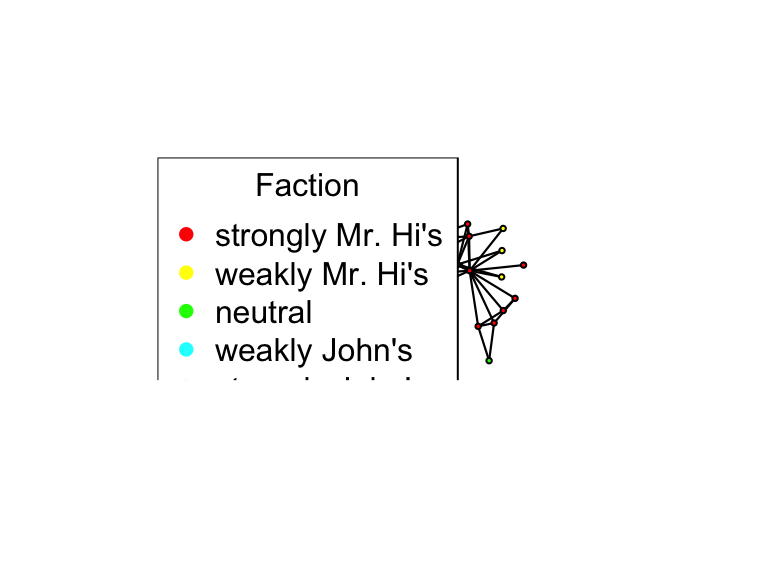
\includegraphics{SNA_BOOK_files/figure-latex/unnamed-chunk-41-1.pdf}

and consider the following model:

\begin{Shaded}
\begin{Highlighting}[]
\NormalTok{model}\FloatTok{.3} \NormalTok{<-}\StringTok{ }\NormalTok{y ~}\StringTok{ }\NormalTok{edges +}\StringTok{ }
\StringTok{               }\KeywordTok{nodematch}\NormalTok{(}\StringTok{"faction.id"}\NormalTok{) +}
\StringTok{               }\KeywordTok{gwesp}\NormalTok{(}\DataTypeTok{decay =} \KeywordTok{log}\NormalTok{(}\DecValTok{2}\NormalTok{), }\DataTypeTok{fixed =} \OtherTok{TRUE}\NormalTok{)}
\end{Highlighting}
\end{Shaded}

\section{Prior specification}\label{prior-specification}

We can also set up the prior mean and variance/covariance structure. The
prior distribution used by the \texttt{Bergm} package is the normal
distribution. In this case, we set the prior mean to be
\(\bar{\theta} = (-1, 0.5, 0)\) (corresponding to negative density and
positive density withing factions and positive transitivity) and the
covariance matrix of each model to be a diagonal matrix with every entry
equal to \(4\). So \[
\theta \sim N \left(\begin{bmatrix}
-1\\ 
0.5\\ 
0.5
\end{bmatrix},
\begin{bmatrix}
4 & 0 & 0\\ 
0 & 4 & 0\\ 
0 & 0 & 4
\end{bmatrix}
\right)
\]

\begin{Shaded}
\begin{Highlighting}[]
\NormalTok{mean.prior <-}\StringTok{ }\KeywordTok{c}\NormalTok{(-}\DecValTok{1}\NormalTok{, }\FloatTok{0.5}\NormalTok{, }\FloatTok{0.5}\NormalTok{)}
\NormalTok{sigma.prior <-}\StringTok{ }\KeywordTok{diag}\NormalTok{(}\DecValTok{4}\NormalTok{, }\DecValTok{3}\NormalTok{)}
\end{Highlighting}
\end{Shaded}

To implement the Bayesian parameter inference procedure we can use the
\texttt{bergm} function:

\begin{Shaded}
\begin{Highlighting}[]
\NormalTok{post <-}\StringTok{ }\KeywordTok{bergm}\NormalTok{(model}\FloatTok{.3}\NormalTok{, }
              \DataTypeTok{aux.iters =} \DecValTok{2000}\NormalTok{, }\CommentTok{# number of iterations for step 1.ii}
              \DataTypeTok{burn.in =} \DecValTok{100}\NormalTok{, }\CommentTok{# number of burnin iterations for each chain}
              \DataTypeTok{main.iters =} \DecValTok{3000}\NormalTok{, }\CommentTok{# number of iterations for each chain (after burnin)}
              \DataTypeTok{nchains =} \DecValTok{5}\NormalTok{, }\CommentTok{# number of chains}
              \DataTypeTok{gamma =} \FloatTok{0.8}\NormalTok{, }\CommentTok{# gamma parameter (tuned to get ~20% acceptance probability)}
              \DataTypeTok{mean.prior =} \NormalTok{mean.prior,}
              \DataTypeTok{sigma.prior =} \NormalTok{sigma.prior)}
\end{Highlighting}
\end{Shaded}

It is possible to visualise the results of the MCMC estimation by using
the \texttt{bergm.output} function which is based on the \texttt{coda}
package:

\begin{Shaded}
\begin{Highlighting}[]
\KeywordTok{bergm.output}\NormalTok{(post)}
\end{Highlighting}
\end{Shaded}

\begin{verbatim}
## 
##  Posterior Density Estimate for Model: y ~ edges + nodematch("faction.id") + gwesp(decay = log(2), fixed = TRUE) 
##  
##                                              Mean        SD    Naive SE
## theta1 (edges)                         -3.2221441 0.2548631 0.002080948
## theta2 (nodematch.faction.id)           1.0492332 0.2318037 0.001892669
## theta3 (gwesp.fixed.0.693147180559945)  0.6070649 0.1359139 0.001109732
##                                        Time-series SE
## theta1 (edges)                            0.012117759
## theta2 (nodematch.faction.id)             0.011372732
## theta3 (gwesp.fixed.0.693147180559945)    0.006532328
## 
##                                              2.5%        25%        50%
## theta1 (edges)                         -3.7453945 -3.3850316 -3.2117128
## theta2 (nodematch.faction.id)           0.5937836  0.8970344  1.0494414
## theta3 (gwesp.fixed.0.693147180559945)  0.3594777  0.5150651  0.6046604
##                                              75%      97.5%
## theta1 (edges)                         -3.052811 -2.7196526
## theta2 (nodematch.faction.id)           1.205293  1.5186659
## theta3 (gwesp.fixed.0.693147180559945)  0.695165  0.8978658
## 
##  Acceptance rate: 0.1824667 
##  
## 
\end{verbatim}

\section{Bayesian goodness of fit
diagnostics}\label{bayesian-goodness-of-fit-diagnostics}

The \texttt{bgof} function provides a useful tool for assessing Bayesian
goodness-of-fit so as to examine the fit of the data to the posterior
model obtained by the \texttt{bergm} function. The observed network data
\(y\) are compared with a set of networks \(y_1, y_2, \dots, y_S\)
simulated from \(S\) independent realisations
\(\theta_1, \theta_2,\dots,\theta_S\) of the posterior density estimate.
This comparison is made in terms of high-level characteristics
\(g(\cdot)\) such as higher degree distributions, etc.
\citep{hun:goo:han08}.

\begin{Shaded}
\begin{Highlighting}[]
\KeywordTok{bgof}\NormalTok{(post, }\DataTypeTok{aux.iters =} \DecValTok{5000}\NormalTok{, }\DataTypeTok{n.deg =} \DecValTok{15}\NormalTok{, }\DataTypeTok{n.dist =} \DecValTok{9}\NormalTok{, }\DataTypeTok{n.esp =} \DecValTok{8}\NormalTok{)}
\end{Highlighting}
\end{Shaded}

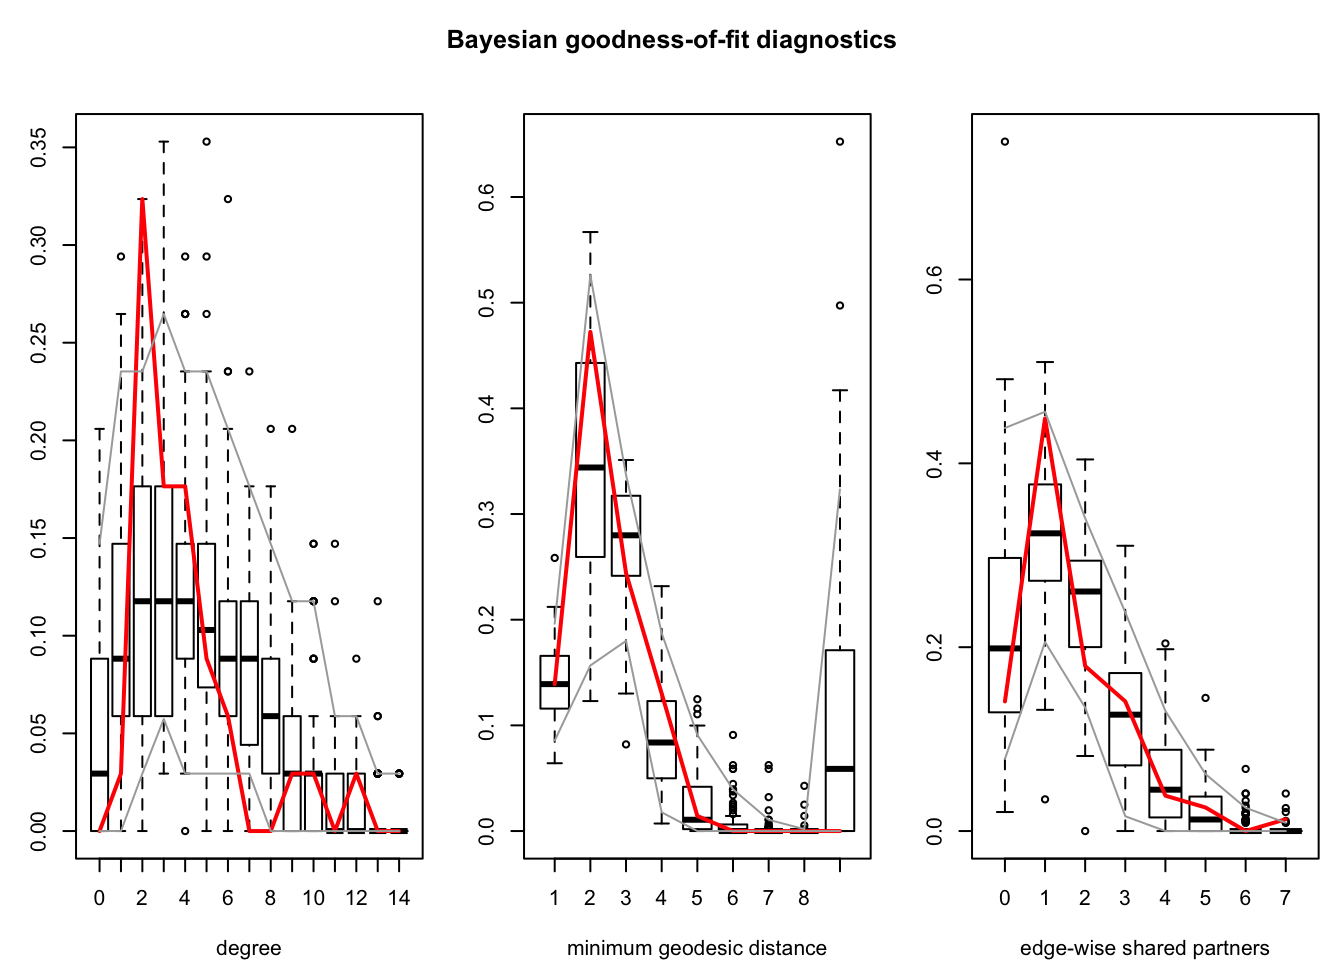
\includegraphics{SNA_BOOK_files/figure-latex/unnamed-chunk-46-1.pdf}

The red line displays the goodness of fit statistics for the observed
data together with boxplots of goodness of fit statistics based on
\(100\) simulated networks from the estimated posterior distribution.

\bibliography{packages.bib,book.bib}


\end{document}
